\clearpage
\section{Casi d'uso}\label{CasiDUso}
Questa sezione elenca le funzionalità offerte da \progetto\ descritte attraverso il linguaggio \gloss{UML}.
\progetto\ può essere visto come l'insieme di più sottosistemi che verranno in seguito elencati e che sono stati descritti in modo molto generale anche attraverso la Figura \ref{fig:butterfly}.\par
Questa mostra in maniera un po' più chiarificante la suddivisione e ne facilita l'analisi per la stesura dei casi d'uso.
Abbiamo quindi come attori non soltanto le applicazioni che mandano messaggi al sistema, ma anche componenti quali i vari Producer e Consumer che interagiscono col Gestore Personale. \par
All'interno dei casi d'uso il termine ``sistema'' è inteso come l'intera applicazione \progetto, mentre ``piattaforma di messaggistica'' fa sempre riferimento a Telegram o Email, il termine ``persona di fiducia'' indica la persona a cui inoltrare le proprie notifiche nei giorni in cui non si è disponibili e con ``indisponibilità'' e ``irreperibilità'' di una persona si intendono proprio quei giorni in cui una persona non è raggiungibile nè disponibile per proseguire con le proprie mansioni e quindi non vuole ricevere notifiche. \par
Il termine ``identificativo'' fa riferimento indifferentemente al contatto Email o all'ID Telegram.
	
	\subsection{Attori}
	\begin{itemize}
		\item Redmine
		\item GitLab
		\item Producer Redmine
		\item Producer GitLab
		\item Utente non acceduto
		\item Utente non registrato
		\item Utente (inteso come acceduto e registrato nel sistema)
		\item Consumer Telegram
		\item Consumer Email
		\item Telegram
		\item Email
	\end{itemize}

	\subsection{Sistemi e sottosistemi}
	Per indicare i vari sottosistemi nei codici dei casi d'uso sono allegati delle sigle per rendere più chiara la posizione del caso d'uso all'interno di \progetto.
	\begin{itemize}
		%\item \textbf{B}: \progetto.
		\item \textbf{PR}: Producer Redmine.
		\item \textbf{PG}: Producer GitLab.
		\item \textbf{GP}: Gestore Personale.
		\item \textbf{CT}: Consumer telegram.
		\item \textbf{CE}: Consumer Email.
		\item \textbf{BT}: bot Telegram.
		\item \textbf{SE}: server Email.
	\end{itemize}

	\clearpage

	\subsection{Elenco casi d'uso}

%TODO: da ricordarsi: se qualcuno è offline, c'è la possibilità che il messaggio venga perso.

\newcounter{uccount}
\newcounter{subuccount}[uccount]
\newcounter{subsubuccount}[subuccount]
\newcounter{subsubsubuccount}[subsubuccount]

%\stepcounter{uccount}
%
%\subsubsection{UC\theuccount-PR - Redmine invia segnalazione al Producer Redmine}
%    \begin{figure}[H]
%		\centering
%		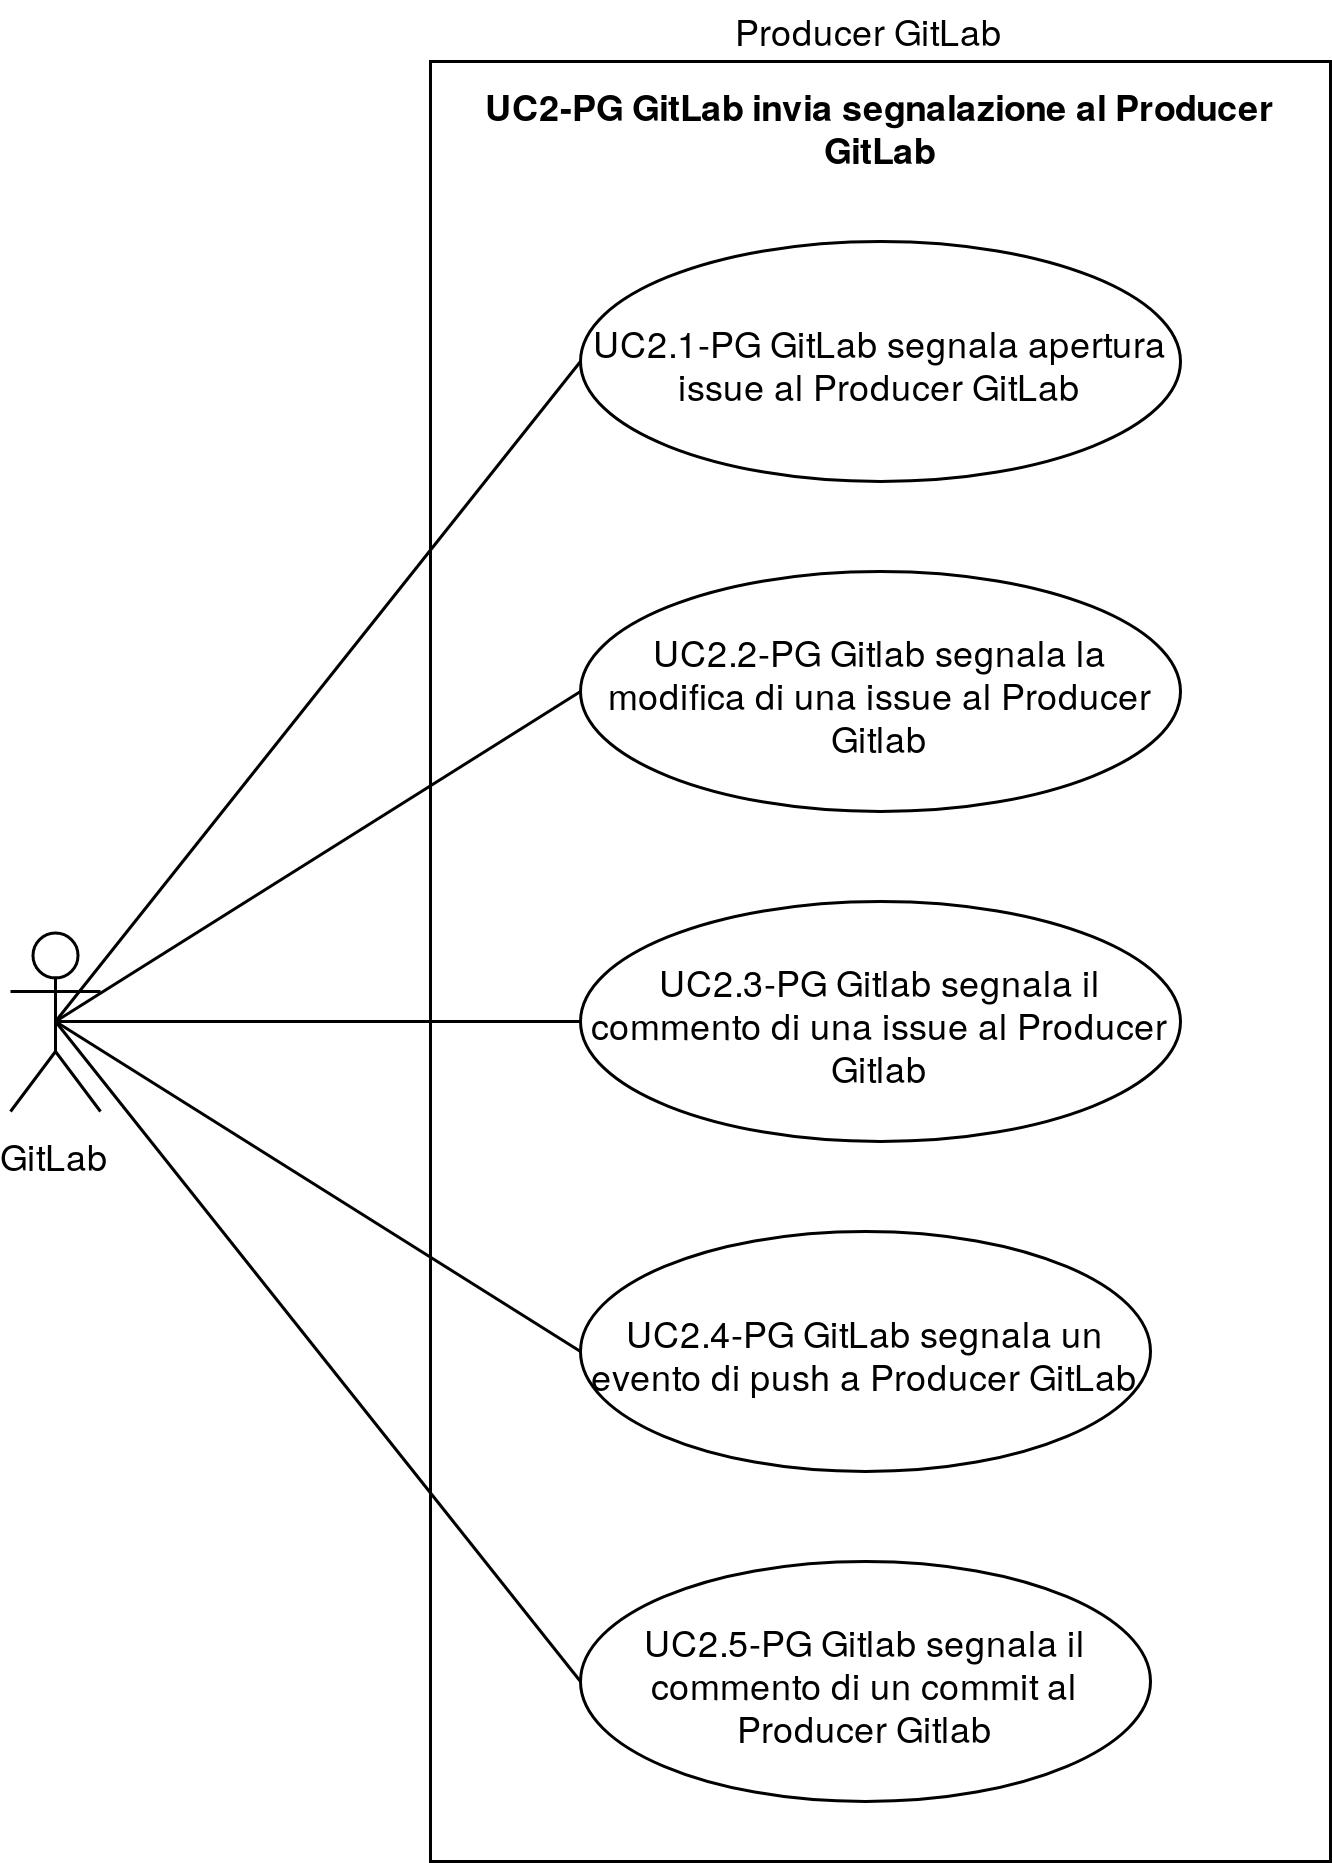
\includegraphics[width=0.5\textwidth]{img/casi_d'uso/UC2.png}\\
%		\caption{UC\theuccount-PR - Redmine segnala apertura issue al Producer Redmine}
%	\end{figure}
\begin{itemize}
	\item \textbf{Codice}: UC\theuccount-PR.
	\item \textbf{Titolo}: Redmine invia segnalazione al Producer Redmine.
	\item \textbf{Attori primari}: Redmine.
	\item \textbf{Descrizione}: Redmine invia a \progetto\ una segnalazione.
	\item \textbf{Precondizione}: su Redmine viene eseguita una operazione che scaturisce una
	segnalazione da inviare a \progetto.
	\item \textbf{Postcondizione}: il Producer Redmine riceve la segnalazione da Redmine.
	\item \textbf{Scenario principale}: 
	\begin{enumerate}
		\item Viene eseguita un'operazione
		\item Redmine procede all'invio della segnalazione al Producer Redmine
	\end{enumerate}
	
\end{itemize}

\stepcounter{subuccount}

\subsubsection{UC\theuccount.\thesubuccount-PR - Redmine segnala apertura issue al Producer Redmine}
%    \begin{figure}[H]
%		\centering
%		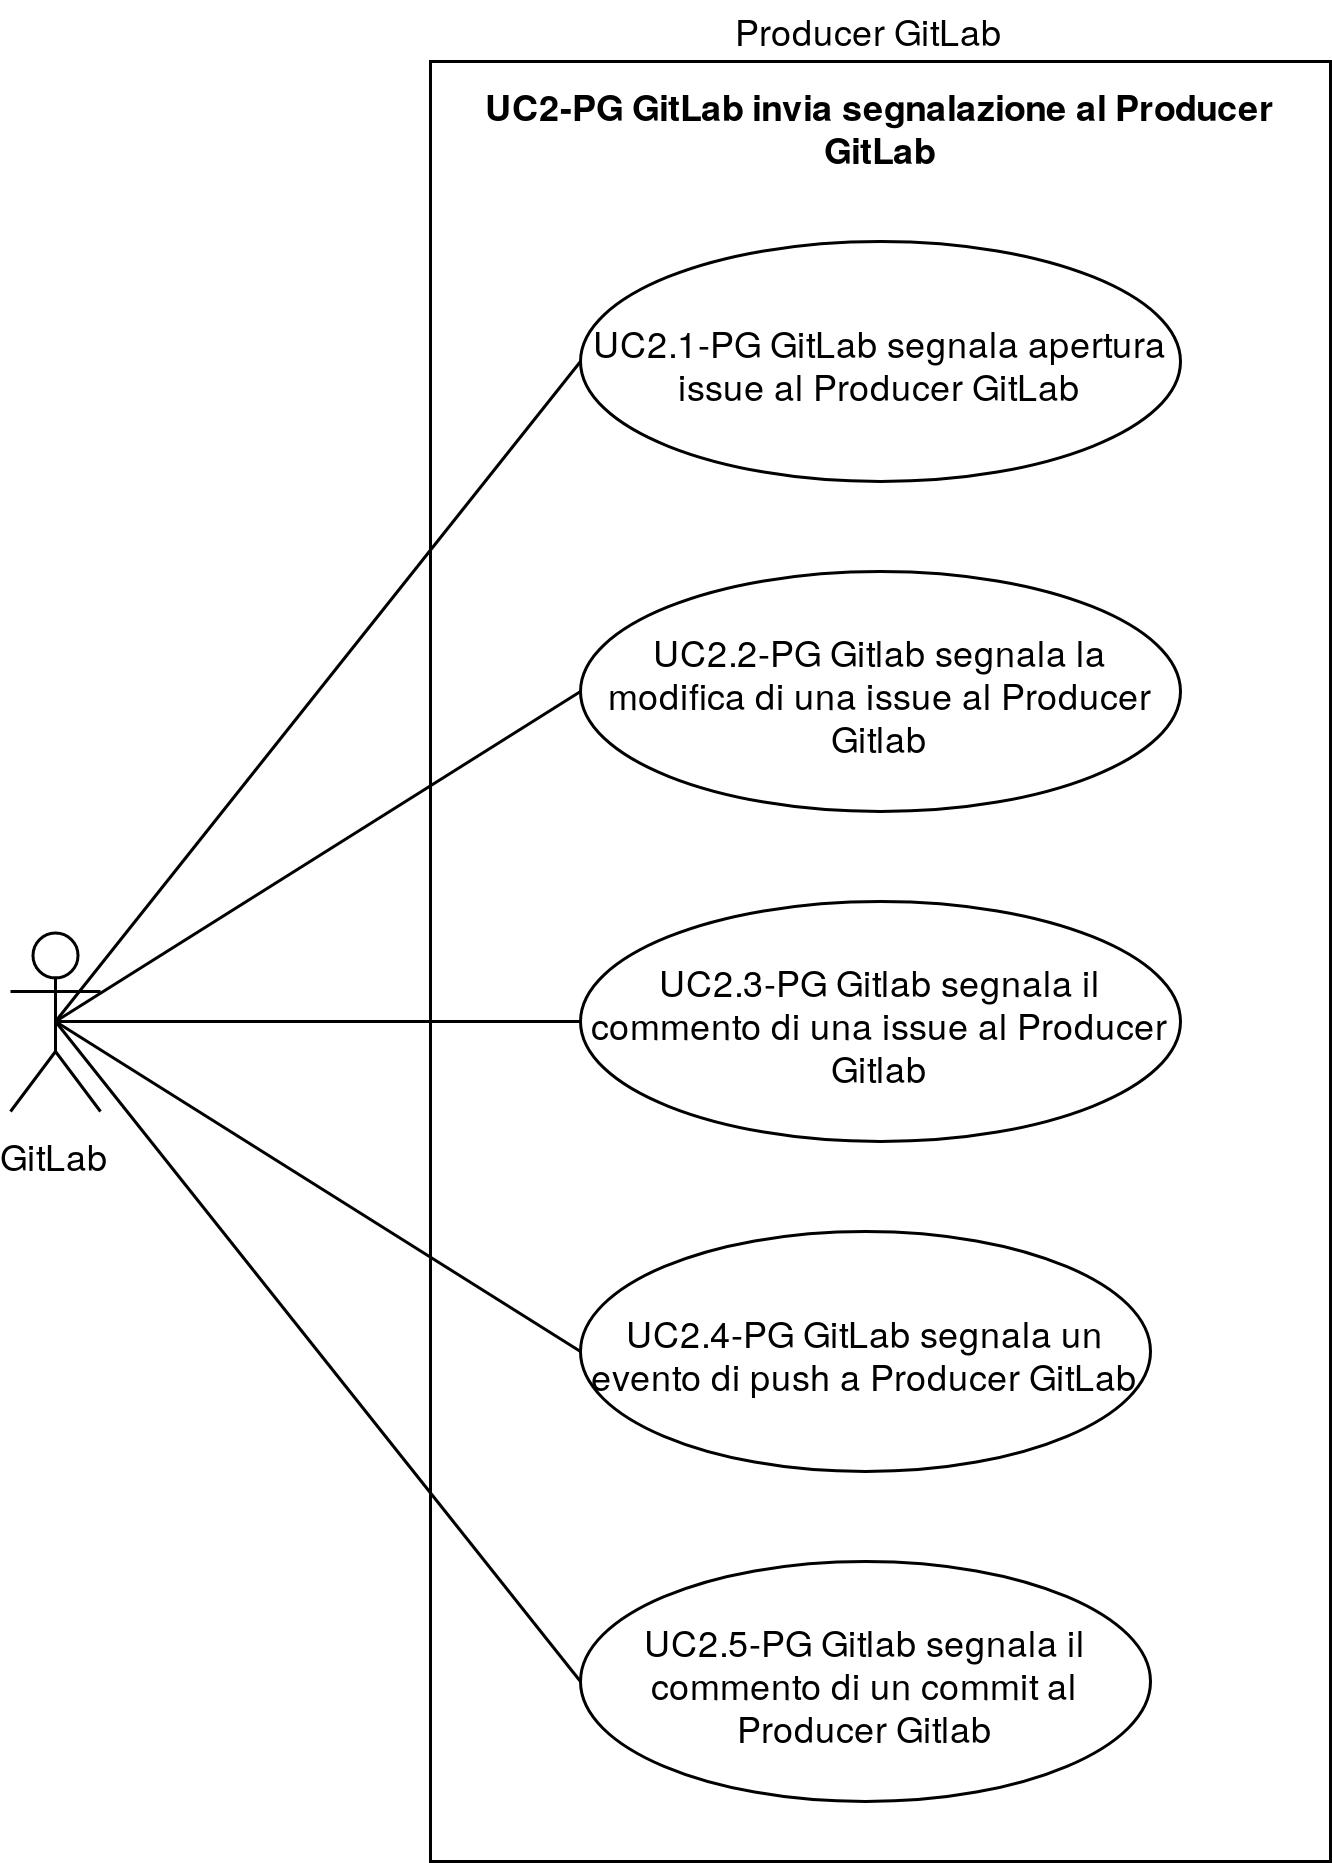
\includegraphics[width=0.5\textwidth]{img/casi_d'uso/UC2.png}\\
%		\caption{UC\theuccount-PR - Redmine segnala apertura issue al Producer Redmine}
%	\end{figure}
\begin{itemize}
	\item \textbf{Codice}: UC\theuccount-PR.
	\item \textbf{Titolo}: Redmine segnala apertura issue al Producer Redmine.
	\item \textbf{Attori primari}: Redmine.
	\item \textbf{Descrizione}: Redmine segnala a \progetto\ l'apertura di una nuova issue tramite webhook.
	
	L'apertura di una issue in un particolare progetto su Redmine contiene i seguenti campi di interesse:
	\begin{itemize}
		\item Status
		\item Tracker
		\item Subject
		\item Priority e opzionalmente:
		\begin{itemize}
			\item Description
			\item Assignee
		\end{itemize}
	\end{itemize}
	Il campo status conterrà sempre al suo interno ``opened''.
	\item \textbf{Precondizione}: Viene aperta una issue su Redmine da
	segnalare a \progetto.
	\item \textbf{Postcondizione}: il Producer Redmine riceve la segnalazione da Redmine.
	\item \textbf{Scenario principale}: 
	\begin{enumerate}
		\item Viene aperta una nuova issue su Redmine
		\item Redmine procede all'invio della segnalazione di issue al Producer Redmine
	\end{enumerate}
	
\end{itemize}

\stepcounter{subuccount}

\subsubsection{UC\theuccount.\thesubuccount-PR - Redmine segnala la modifica di una issue al Producer Redmine}
%	\begin{figure}[H]
%		\centering
%		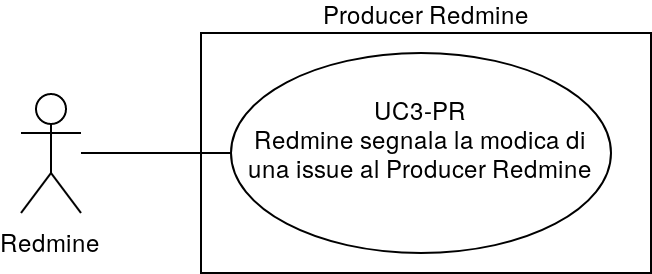
\includegraphics[width=0.5\textwidth]{img/casi_d'uso/UC3.png}\\
%		\caption{UC\theuccount-PR - Redmine segnala la modifica di una issue al Producer Redmine}
%	\end{figure}
\begin{itemize}
	\item \textbf{Codice}: UC\theuccount-PR.
	\item \textbf{Titolo}: Redmine segnala la modifica di una issue al Producer Redmine.
	\item \textbf{Attori primari}: Redmine.
	\item \textbf{Descrizione}: quando una issue viene modificata, l'invio di tale segnalazione
	avviene da parte di Redmine tramite webhook.
	I campi di interesse sono gli stessi dell'apertura di una issue, con la differenza che necessariamente il campo status contiene ora ``updated''.
	\item \textbf{Precondizione}: Viene modificata una issue già aperta su un
	progetto di Redmine da segnalare a \progetto.
	\item \textbf{Postcondizione}: il Producer Redmine riceve la segnalazione da Redmine.
	\item \textbf{Scenario principale}: 
	\begin{enumerate}
		\item Viene modificata una issue già esistente su Redmine
		\item Redmine procede all'invio della segnalazione di modifica issue al Producer Redmine
	\end{enumerate}
	
\end{itemize}

\stepcounter{subuccount}

\subsubsection{UC\theuccount.\thesubuccount-PR - Redmine segnala il commento di una issue al Producer Redmine}
%	\begin{figure}[H]
%		\centering
%		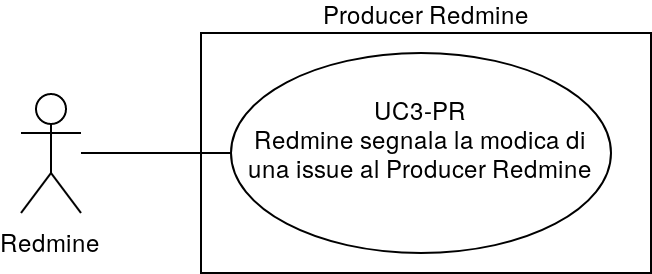
\includegraphics[width=0.5\textwidth]{img/casi_d'uso/UC3.png}\\
%		\caption{UC\theuccount-PR - Redmine segnala la modifica di una issue al Producer Redmine}
%	\end{figure}
\begin{itemize}
	\item \textbf{Codice}: UC\theuccount.\thesubuccount-PR.
	\item \textbf{Titolo}: Redmine segnala il commento di una issue al Producer Redmine.
	\item \textbf{Attori primari}: Redmine.
	\item \textbf{Descrizione}: quando una issue viene commentata, l'invio di tale segnalazione
	avviene da parte di Redmine tramite webhook.
	I campi di interesse sono gli stessi della modifica di una issue, con la differenza che necessariamente il campo status contiene ora ``updated''.
	\item \textbf{Precondizione}: Viene modificata una issue già aperta su un
	progetto di Redmine da segnalare a \progetto.
	\item \textbf{Postcondizione}: il Producer Redmine riceve la segnalazione da Redmine.
	\item \textbf{Scenario principale}: 
	\begin{enumerate}
		\item Viene modificata una issue già esistente su Redmine
		\item Redmine procede all'invio della segnalazione di modifica issue al Producer Redmine
	\end{enumerate}
	
\end{itemize}


\stepcounter{uccount}
%\clearpage
\subsubsection{UC\theuccount-PG - GitLab invia segnalazione al Producer GitLab}
	\begin{figure}[H]
		\centering
		\includegraphics[width=0.8\textwidth]{img/casi_d'uso/UC\theuccount.png}\\
		\caption{UC2-PG - GitLab invia segnalazione al Producer GitLab}
	\end{figure}
\begin{itemize}
    \item \textbf{Codice}: UC\theuccount-PG.
    \item \textbf{Titolo}: GitLab invia segnalazione al Producer GitLab.
    \item \textbf{Attori primari}: GitLab.
    \item \textbf{Descrizione}: GitLab invia una segnalazione tramite webhook a \progetto.
    \item \textbf{Precondizione}: su GitLab viene eseguita una operazione che scaturisce una
    segnalazione da inviare a \progetto.
    \item \textbf{Postcondizione}: il Producer GitLab riceve la segnalazione da GitLab.
    \item \textbf{Scenario principale}:
    \begin{enumerate}
        \item Viene eseguita un'operazione
        \item GitLab procede all'invio della segnalazione al Producer GitLab
        \item Il Producer GitLab riceve la segnalazione
    \end{enumerate}

\end{itemize}

\stepcounter{subuccount}

\subsubsection{UC\theuccount.\thesubuccount-PG - GitLab segnala apertura issue al Producer GitLab}
\begin{itemize}
    \item \textbf{Codice}: UC\theuccount.\thesubuccount-PG.
    \item \textbf{Titolo}: GitLab segnala apertura issue al Producer GitLab.
    \item \textbf{Attori primari}: GitLab.
    \item \textbf{Descrizione}: GitLab segnala l'apertura di una nuova issue tramite webhook a \progetto.
    L'apertura di una issue su GitLab contiene:
    \begin{itemize}
        \item Object kind
        \item Action
        \item Project
        \item Title e opzionalmente:
        \begin{itemize}
            \item Label
            \item Milestone
            \item Assignees
            \item Due Date
        \end{itemize}
    \end{itemize}
    Il campo object kind ci permette di capire il tipo di oggetto. In questo caso infatti contiene ``issue'', mentre il campo action ha ``open''.
    \item \textbf{Precondizione}: su GitLab viene eseguita una operazione che scaturisce una
    segnalazione da inviare a \progetto.
    \item \textbf{Postcondizione}: il Producer GitLab riceve la segnalazione di apertura issue da GitLab.
    \item \textbf{Scenario principale}:
    \begin{enumerate}
        \item Viene aperta una nuova issue su GitLab
        \item GitLab procede all'invio della segnalazione di issue al Producer GitLab
        \item Il Producer GitLab riceve la segnalazione di apertura issue
    \end{enumerate}

\end{itemize}

\stepcounter{subuccount}

\subsubsection{UC\theuccount.\thesubuccount-PG - Gitlab segnala la modifica di una issue al Producer Gitlab}
\begin{itemize}
    \item \textbf{Codice}: UC\theuccount.\thesubuccount-PG.
    \item \textbf{Titolo}: Gitlab segnala la modifica di una issue al Producer Gitlab.
    \item \textbf{Attori primari}: GitLab.
    \item \textbf{Descrizione}: GitLab segnala la modifica di una issue esistente tramite webhook a
    \newline \progetto.
    I campi di interesse sono gli stessi dell'apertura issue, con la differenza che il campo action contiene ``udpate''.
    \item \textbf{Precondizione}: su GitLab viene eseguita una operazione che scaturisce una
    segnalazione da inviare a \progetto.
    \item \textbf{Postcondizione}: il Producer GitLab riceve la segnalazione di modifica issue da GitLab.
    \item \textbf{Scenario principale}:
    \begin{enumerate}
        \item Viene modificata una issue già esistente su GitLab
        \item GitLab procede all'invio della segnalazione di modifica issue al Producer GitLab
        \item Il Producer GitLab riceve la segnalazione di modifica issue
    \end{enumerate}

\end{itemize}

\stepcounter{subuccount}

\subsubsection{UC\theuccount.\thesubuccount-PG - Gitlab segnala il commento di una issue al Producer Gitlab}
\begin{itemize}
    \item \textbf{Codice}: UC\theuccount.\thesubuccount-PG.
    \item \textbf{Titolo}: Gitlab segnala il commento di una issue al Producer Gitlab.
    \item \textbf{Attori primari}: GitLab.
    \item \textbf{Descrizione}: GitLab segnala il commento di una issue esistente tramite webhook a \progetto.
    I campi di interesse sono gli stessi dell'apertura issue, con la differenza che il campo action contiene ``issue-note''.
    \item \textbf{Precondizione}: su GitLab viene eseguita una operazione che scaturisce una
    segnalazione da inviare a \progetto.
    \item \textbf{Postcondizione}: il Producer GitLab riceve la segnalazione di commento issue da GitLab.
    \item \textbf{Scenario principale}:
    \begin{enumerate}
        \item Viene commentata una issue già esistente su GitLab
        \item GitLab procede all'invio della segnalazione di commento issue al Producer GitLab
        \item \item Il Producer GitLab riceve la segnalazione di commento di una issue
    \end{enumerate}

\end{itemize}

\stepcounter{subuccount}

\subsubsection{UC\theuccount.\thesubuccount-PG - GitLab segnala un evento di push a Producer GitLab}
\begin{itemize}
\item \textbf{Codice}: UC\theuccount.\thesubuccount-PG.
\item \textbf{Titolo}: GitLab segnala un evento di push a Producer GitLab.
\item \textbf{Attori primari}: GitLab.
\item \textbf{Descrizione}: GitLab segnala un evento di push tramite webhook a \progetto. L'evento di push può essere composto da uno o più commit.
I campi di interesse sono:
\begin{itemize}
    \item Object kind
    \item Project
    \item Repository
    \item Commits
\end{itemize}
E in questo caso il campo object kind contiene ``push''.
\item \textbf{Precondizione}: su GitLab viene eseguita una operazione che scaturisce una
segnalazione da inviare a \progetto.
\item \textbf{Postcondizione}: il Producer GitLab riceve la segnalazione di push da GitLab.
\item \textbf{Scenario principale}:
\begin{enumerate}
    \item Viene effettuato un push in GitLab
    \item GitLab procede all'invio della segnalazione di push al Producer GitLab
    \item Il Producer GitLab riceve la segnalazione dell'evento di push
\end{enumerate}

\end{itemize}

\stepcounter{subuccount}

\subsubsection{UC\theuccount.\thesubuccount-PG - Gitlab segnala il commento di un commit al Producer Gitlab}
\begin{itemize}
    \item \textbf{Codice}: UC\theuccount.\thesubuccount-PG.
    \item \textbf{Titolo}: Gitlab segnala il commento di un commit al Producer Gitlab.
    \item \textbf{Attori primari}: GitLab.
    \item \textbf{Descrizione}: GitLab segnala il commento di un commit esistente tramite webhook a \progetto.
    I campi di interesse sono gli stessi dell'apertura issue, con la differenza che il campo action contiene ``commit-note''.
    \item \textbf{Precondizione}: su GitLab viene eseguita una operazione che scaturisce una
    segnalazione da inviare a \progetto.
    \item \textbf{Postcondizione}: il Producer GitLab riceve la segnalazione di commento di commit da GitLab.
    \item \textbf{Scenario principale}:
    \begin{enumerate}
        \item Viene commentato un commit già esistente su GitLab
        \item GitLab procede all'invio della segnalazione di commento commit al Producer GitLab
        \item Il Producer GitLab riceve la segnalazione di commento di un commit
    \end{enumerate}

\end{itemize}


\stepcounter{uccount}
%\clearpage
	\subsubsection{UC\theuccount-PR - Redmine segnala la modifica di una issue al Producer Redmine}
	\begin{figure}[H]
		\centering
		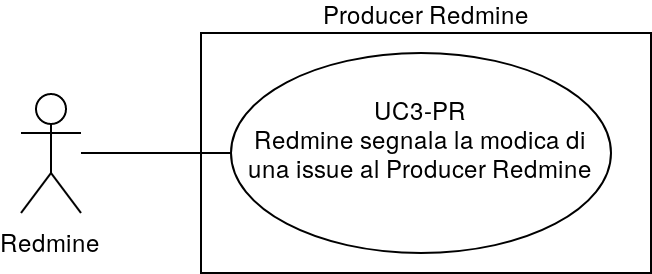
\includegraphics[width=0.7\textwidth]{img/casi_d'uso/UC3.png}\\
		\caption{UC\theuccount-PR - Redmine segnala la modifica di una issue al Producer Redmine}
	\end{figure}
	\begin{itemize}
		\item \textbf{Codice}: UC\theuccount-PR.
		\item \textbf{Titolo}: Redmine segnala la modifica di una issue al Producer Redmine.
		\item \textbf{Attori primari}: Redmine.
		\item \textbf{Descrizione}: quando una issue viene modificata, l'invio di tale segnalazione avviene da parte di Redmine tramite webhook, .
		\item \textbf{Precondizione}: Viene modificata una issue già aperta su un
		progetto di Redmine da segnalare a \progetto.
		\item \textbf{Postcondizione}: il Producer Redmine riceve la segnalazione da Redmine.
		\item \textbf{Scenario principale}: 
		\begin{enumerate}
			\item Viene modificata una issue già esistente su Redmine
			\item Redmine procede all'invio della segnalazione di modifica issue al Producer Redmine
		\end{enumerate}
		
	\end{itemize}

\stepcounter{uccount}
%\clearpage
\subsubsection{UC\theuccount-GP - Producer GitLab invia messaggio al Gestore Personale}
	\begin{figure}[H]
		\centering
		\includegraphics[width=0.8\textwidth]{img/casi_d'uso/UC\theuccount.png}\\
		\caption{UC\theuccount-GP - Producer GitLab invia messaggio al Gestore Personale}
	\end{figure}
	\begin{itemize}
		\item \textbf{Codice}: UC\theuccount-GP.
		\item \textbf{Titolo}: Producer GitLab invia messaggio al Gestore Personale.
		\item \textbf{Attori primari}: Producer GitLab.
		\item \textbf{Descrizione}: il Producer GitLab, dopo aver ricevuto una segnalazione da GitLab, elabora un messaggio da inviare al Gestore Personale. \\ Il messaggio elaborato conterrà i campi:
		\begin{itemize}
			\item App
			\item Object\_kind
			\item Title
			\item Project\_id
			\item Project\_name
			\item Author
			\item Assignees
			\item Action
			\item Description
			\item Labels
			\item Update
		\end{itemize}
        Se il Producer Gitlab riceve una segnalazione che non è in grado di analizzare, questa viene scartata.
		\item \textbf{Precondizione}: il Producer GitLab ha ricevuto una segnalazione da GitLab.
		\item \textbf{Postcondizione}: il Producer GitLab ha inviato al Gestore Personale il messaggio elaborato.
		\item \textbf{Scenario principale}:
		\begin{enumerate}
			\item Il Producer GitLab riceve una segnalazione da GitLab
			\item Il Producer GitLab prepara il messaggio in modo che venga inserito correttamente nel Gestore Personale
			\item Il Poducer GitLab invia il messaggio al Gestore Personale
            \item Il Gestore Perosonale riceve il messaggio dal Producer GitLab
		\end{enumerate}
	\end{itemize}

	\stepcounter{subuccount}

	\subsubsection{UC\theuccount.\thesubuccount-GP - Producer GitLab invia messaggio di push al Gestore Personale}

		\begin{itemize}
			\item \textbf{Codice}: UC\theuccount.\thesubuccount-GP.
			\item \textbf{Titolo}: Producer GitLab invia uno o più messaggi di commit al Gestore Personale.
			\item \textbf{Attori primari}: Producer GitLab.
			\item \textbf{Descrizione}: il Producer GitLab, dopo aver ricevuto una segnalazione di push da  \newline GitLab, suddivide la segnalazione per i commit in più messaggi che verranno catalogati sotto il Topic ``commits''.
			\item \textbf{Precondizione}: il Producer GitLab ha ricevuto una segnalazione da GitLab.
			\item \textbf{Postcondizione}: il Producer GitLab ha inviato uno o più messaggi di commit.
			\item \textbf{Scenario principale}:
			\begin{enumerate}
				\item Il Producer GitLab riceve la segnalazione di un push da GitLab
				\item Il Producer GitLab prepara i messaggi in modo che vengano inseriti correttamente nel Gestore Personale
				\item Il Producer GitLab invia i messaggi di
				commit al Gestore Personale
                \item Il Gestore Personale riceve i messaggi di commit
			\end{enumerate}
%			\item \textbf{Estensioni}:
%			\begin{enumerate}
%				\item Se ci sono dei messaggi non validi, questi vengono scartati [UC\theuccount.6-GP].
%			\end{enumerate}
		\end{itemize}

	\stepcounter{subuccount}

	\subsubsection{UC\theuccount.\thesubuccount-GP - Producer GitLab invia messaggio di una nuova issue al Gestore Personale}

	\begin{itemize}
		\item \textbf{Codice}: UC\theuccount.\thesubuccount-GP.
		\item \textbf{Titolo}: Producer GitLab invia messaggio di una nuova issue al Gestore Personale.
		\item \textbf{Attori primari}: Producer GitLab.
		\item \textbf{Descrizione}: il Producer GitLab, dopo aver ricevuto una segnalazione di una nuova issue da GitLab, elabora il messaggio da inoltrare al Gestore Personale.
		\item \textbf{Precondizione}: il Producer GitLab ha ricevuto una segnalazione da GitLab.
		\item \textbf{Postcondizione}: il Producer GitLab ha inviato al Gestore Personale il messaggio
		elaborato di nuova issue.
		\item \textbf{Scenario principale}:
		\begin{enumerate}
			\item Il Producer GitLab riceve la segnalazione di una nuova issue da GitLab
			\item Il Producer GitLab prepara il messaggio di una nuova issue in modo che venga inserito correttamente
			nel Gestore Personale
			\item Il Producer GitLab invia il messaggio di una nuova issue al Gestore Personale
			\item Il Gestore Personale riceve il messaggio di apertura issue dal Producer GitLab
		\end{enumerate}
%		\item \textbf{Estensioni}:
%		\begin{enumerate}
%			\item Se ci sono dei messaggi non validi, questi vengono scartati [UC\theuccount.6-GP].
%		\end{enumerate}
	\end{itemize}

	\stepcounter{subuccount}

	\subsubsection{UC\theuccount.\thesubuccount-GP - Producer GitLab invia messaggio di modifica di una issue al Gestore Personale}
		\begin{itemize}
			\item \textbf{Codice}: UC\theuccount.\thesubuccount-GP.
			\item \textbf{Titolo}: Producer GitLab invia messaggio di modifica di una issue al Gestore Personale.
			\item \textbf{Attori primari}: Producer GitLab.
			\item \textbf{Descrizione}: il Producer GitLab, dopo aver ricevuto una segnalazione di una modifica issue da GitLab, elabora il messaggio da inoltrare al Gestore Personale.
			% Il messaggio, una volta elaborato, conterrà i campi:
			% \begin{itemize}
			% 	\item Project
            %     \item Author
			% 	\item Topic
			% 	\item Subject e opzionalmente:
			% 	\begin{itemize}
			% 		\item Description
			% 		\item Due Date
			% 		\item Milestone
			% 		\item Assignee
			% 	\end{itemize}
			% \end{itemize}
			\item \textbf{Precondizione}: il Producer GitLab ha ricevuto una segnalazione da GitLab.
			\item \textbf{Postcondizione}: il Producer GitLab ha inviato al Gestore Personale il messaggio
			elaborato di modifica issue.
			\item \textbf{Scenario principale}:
			\begin{enumerate}
				\item Il Producer GitLab riceve la segnalazione di issue da GitLab
				\item Il Producer GitLab prepara il messaggio di modifica issue in modo che venga inserito correttamente nel Gestore Personale
				\item Il Producer GitLab invia il messaggio di issue al Gestore Personale
                \item Il Gestore Personale riceve il messaggio di modifica issue dal Producer GitLab
			\end{enumerate}
%			\item \textbf{Estensioni}:
%			\begin{enumerate}
%				\item Se ci sono dei messaggi non validi, questi vengono scartati [UC\theuccount.6-GP].
%			\end{enumerate}
		\end{itemize}

		\stepcounter{subuccount}

		\subsubsection{UC\theuccount.\thesubuccount-GP - Producer GitLab invia messaggio di commento di una issue al Gestore Personale}
		\begin{itemize}
			\item \textbf{Codice}: UC\theuccount.\thesubuccount-GP.
			\item \textbf{Titolo}: Producer GitLab invia messaggio di commento di una issue al Gestore Personale.
			\item \textbf{Attori primari}: Producer GitLab.
			\item \textbf{Descrizione}: il Producer GitLab, dopo aver ricevuto una segnalazione di commento di una issue da GitLab, elabora il messaggio da inoltrare al Gestore Personale.
			\item \textbf{Precondizione}: il Producer GitLab ha ricevuto una segnalazione da GitLab.
			\item \textbf{Postcondizione}: il Producer GitLab ha inviato al Gestore Personale il messaggio
			elaborato di commento issue.
			\item \textbf{Scenario principale}:
			\begin{enumerate}
				\item Il Producer GitLab riceve la segnalazione di commento issue da GitLab
				\item Il Producer GitLab prepara il messaggio di commento issue in modo che venga inserito correttamente nel Gestore Personale
				\item Il Producer GitLab invia il messaggio di commento issue al Gestore Personale
				\item Il Gestore Personale riceve il messaggio di commento issue dal Producer GitLab
			\end{enumerate}
%			\item \textbf{Estensioni}:
%			\begin{enumerate}
%				\item Se ci sono dei messaggi non validi, questi vengono scartati [UC\theuccount.6-GP].
%			\end{enumerate}
		\end{itemize}

		\stepcounter{subuccount}

		\subsubsection{UC\theuccount.\thesubuccount-GP - Producer GitLab invia messaggio di commento di un commit al Gestore Personale}
		\begin{itemize}
			\item \textbf{Codice}: UC\theuccount.\thesubuccount-GP.
			\item \textbf{Titolo}: Producer GitLab invia messaggio di commento di un commit al Gestore Personale.
			\item \textbf{Attori primari}: Producer GitLab.
			\item \textbf{Descrizione}: il Producer GitLab, dopo aver ricevuto una segnalazione di commento di un commit da GitLab, elabora il messaggio da inoltrare al Gestore Personale.
			\item \textbf{Precondizione}: il Producer GitLab ha ricevuto una segnalazione da GitLab.
			\item \textbf{Postcondizione}: il Producer GitLab ha inviato al Gestore Personale il messaggio
			elaborato di commento commit.
			\item \textbf{Scenario principale}:
			\begin{enumerate}
				\item Il Producer GitLab riceve la segnalazione di commento commit da GitLab
				\item Il Producer GitLab prepara il messaggio di commento commit in modo che venga inserito correttamente nel Gestore Personale
				\item Il Producer GitLab invia il messaggio di commento commit al Gestore Personale
				\item Il Gestore Personale riceve il messaggio di commento issue dal Producer GitLab
			\end{enumerate}
%			\item \textbf{Estensioni}:
%			\begin{enumerate}
%				\item Se ci sono dei messaggi non validi, questi vengono scartati [UC\theuccount.6-GP].
%			\end{enumerate}
		\end{itemize}


\stepcounter{uccount}
%\clearpage
\subsubsection{UC\theuccount-CT - Gestore Personale invia il messaggio finale al Consumer Telegram}
%	\begin{figure}[H]
%		\centering
%		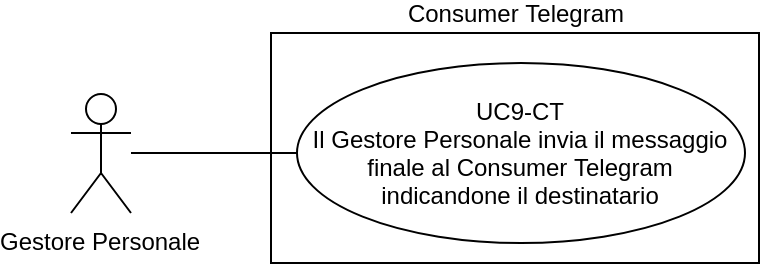
\includegraphics[width=0.6\textwidth]{img/casi_d'uso/UC9.png}\\
%		\caption{UC\theuccount-CT - Gestore Personale invia il messaggio finale al Consumer Telegram}
%	\end{figure}
	\begin{itemize}
		\item \textbf{Codice}: UC\theuccount-CT.
		\item \textbf{Titolo}: Gestore Personale invia il messaggio finale al Consumer Telegram.
		\item \textbf{Attori primari}: Gestore Personale.
		\item \textbf{Descrizione}: il Gestore Personale, dopo aver ricevuto il messaggio elaborato
		dal Producer Redmine o GitLab, controlla i Topic del messaggio, gli utenti iscritti, la loro disponibilità e se la loro preferenza è Telegram.
		Se tutte queste condizioni sono verificate, viene preparato il messaggio finale da inviare successivamente viene inviato al Consumer Telegram. 
		Se il destinatario è iscritto a quel Topic ma non è disponibile, il destinatario viene cambiato con la persona di fiducia. \par
		Il messaggio finale, una volta elaborato, conterrà i campi:
		\begin{itemize}
			\item Id della chat del destinatario
			\item Applicazione di provenienza
			\item Ora di invio
			\item Tipo di segnalazione(commit o issue)
			\item Project
			\item Topic
			\item Subject e opzionalmente
		 	\begin{itemize}
				\item Description
				\item Due date
				\item Milestone
				\item Assignee
			\end{itemize}
		\end{itemize}
		\item \textbf{Precondizione}: il Gestore Personale ha ricevuto il messaggio elaborato dal Producer Redmine o GitLab.
		\item \textbf{Postcondizione}: Il Gestore Personale ha inviato il messaggio finale al Consumer Telegram.
		\item \textbf{Scenario principale}: 
		\begin{enumerate}
			\item ll Gestore Personale riceve un messaggio dal Producer Redmine o dal Producer GitLab
			\item Il Gestore Personale valuta quali utenti sono iscritti al Topic del messaggio ricevuto e se vogliono ricevere il messaggio tramite Telegram
			\item Il Gestore Personale procede all'invio del messaggio finale al Consumer Telegram
		\end{enumerate}
		
	\end{itemize}

\stepcounter{uccount}
%\clearpage
\subsubsection{UC\theuccount-PG - GitLab segnala un evento di push a Producer GitLab}
%	\begin{figure}[H]
%		\centering
%		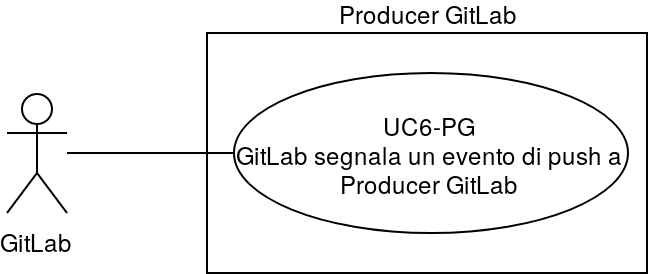
\includegraphics[width=0.5\textwidth]{img/casi_d'uso/UC6.png}\\
%		\caption{UC\theuccount-PG - GitLab segnala un evento di push a Producer GitLab}
%	\end{figure}
	\begin{itemize}
		\item \textbf{Codice}: UC\theuccount-PG.
		\item \textbf{Titolo}: GitLab segnala un evento di push a Producer GitLab.
		\item \textbf{Attori primari}: GitLab.
		\item \textbf{Descrizione}: GitLab segnala un evento di push tramite webhook a \progetto. L'evento di	push può essere composto da uno o più commit.
		I campi di interesse sono:
		\begin{itemize}
			\item Object kind
			\item Project
			\item Repository
			\item Commits
		\end{itemize}
		E in questo caso il campo object kind contiene ``push''.
		\item \textbf{Precondizione}: Viene effettuato un push su GitLab da segnalare a \progetto.
		\item \textbf{Postcondizione}: il Producer GitLab riceve la segnalazione da GitLab.
		\item \textbf{Scenario principale}: 
		\begin{enumerate}
			\item Viene effettuato un push in GitLab
			\item GitLab procede all'invio della segnalazione di push al Producer GitLab
		\end{enumerate}
		
	\end{itemize}

\stepcounter{uccount}
%\clearpage
\subsubsection{UC\theuccount-GP - Producer Redmine invia messaggio al Gestore Personale}
    \begin{figure}[H]
		\centering
		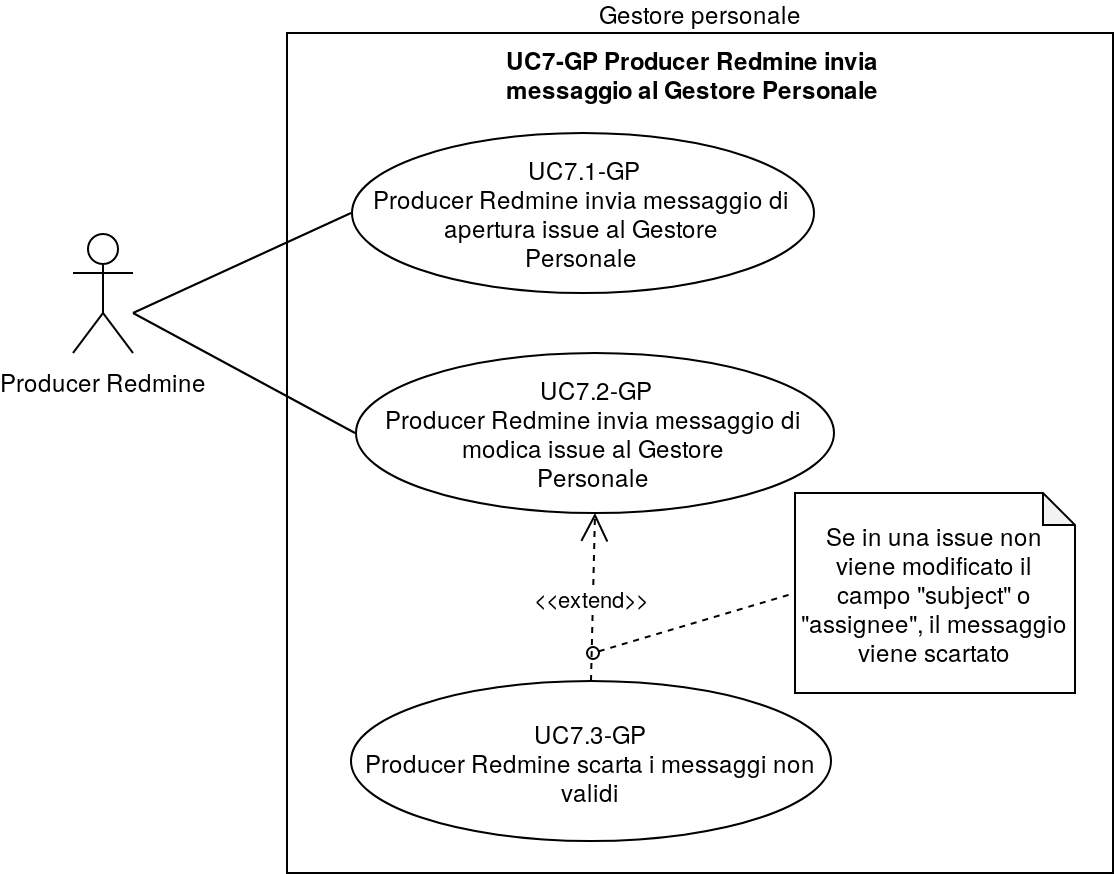
\includegraphics[width=0.8\textwidth]{img/casi_d'uso/UC7.png}\\
		\caption{UC\theuccount-GP - Producer Redmine invia messaggio al Gestore Personale}
	\end{figure}
	\begin{itemize}
		\item \textbf{Codice}: UC\theuccount-GP.
		\item \textbf{Titolo}: Producer Redmine invia messaggio al Gestore Personale.
		\item \textbf{Attori Pimari}: Producer Redmine.
		\item \textbf{Descrizione}: il Producer Redmine, dopo aver ricevuto una
		 segnalazione da Redmine, elabora il messaggio e lo invia al Gestore Personale.
		 Il messaggio finale, una volta terminata l'elaborazione, conterrà i campi:
		 \begin{itemize}
		 	\item Poject
		 	\item Topic
		 	\item Subject e opzionalmente:
		 	\begin{itemize}
		 		\item Description
		 	\end{itemize}
		 \end{itemize}
	 	Il messaggio non può contenere campi errati o mancanti per il corretto funzionamenti di \progetto, perché i campi selezionati sono obbligatori per l'apertura di una issue su Redmine.
		\item \textbf{Pecondizione}: il Producer Redmine ha ricevuto una segnalazione da Redmine.
		\item \textbf{Postcondizione}: il Producer Redmine ha elaborato e inviato al Gestore Personale il messaggio.
		\item \textbf{Scenario GPincipale}: 
		\begin{enumerate}
			\item Il Producer Redmine riceve la segnalazione di issue da Redmine
			\item Il Producer Redmine prepara il messaggio di issue in modo che venga inserito correttamente nel Gestore Personale
			\item Il Producer Redmine invia il messaggio di issue al Gestore Personale
		\end{enumerate}
		
	\end{itemize}
	
	\stepcounter{subuccount}
	\paragraph{UC\theuccount.\thesubuccount-GP - Producer Redmine invia messaggio di apertura issue al Gestore Personale}
	
	\begin{itemize}
		\item \textbf{Codice}: UC\theuccount.\thesubuccount-GP.
		\item \textbf{Titolo}: Producer Redmine invia messaggio di apertura issue al Gestore Personale.
		\item \textbf{Attori Pimari}: Producer Redmine.
		\item \textbf{Descrizione}: il Producer Redmine, dopo aver
		ricevuto una segnalazione di apertura issue da Redmine, elabora il messaggio e lo invia al Gestore Personale.
		Il messaggio finale, una volta terminata l'elaborazione, conterrà i campi:
		\begin{itemize}
			\item Poject
			\item Topic
			\item Subject e opzionalmente:
			\begin{itemize}
				\item Description
			\end{itemize}
		\end{itemize}
		\item \textbf{Pecondizione}: il Producer Redmine ha ricevuto una segnalazione da Redmine.
		\item \textbf{Postcondizione}: il GPoducer Redmine ha elaborato e inviato al Gestore Personale il messaggio di apertura issue.
		\item \textbf{Scenario Pincipale}: 
		\begin{enumerate}
			\item Il Producer Redmine riceve la segnalazione di apertura issue da Redmine
			\item Il Producer Redmine prepara il messaggio in modo che venga inserito correttamente nel Gestore Personale
			\item Il Producer Redmine invia il messaggio di
			apertura issue al Gestore Personale
		\end{enumerate}
		
	\end{itemize}
	
	\stepcounter{subuccount}
	\paragraph{UC\theuccount.\thesubuccount-GP - Producer Redmine invia messaggio di modifica issue al Gestore Personale}
		
		\begin{itemize}
			\item \textbf{Codice}: UC\theuccount.\thesubuccount-GP.
			\item \textbf{Titolo}: Producer Redmine invia messaggio di modifica issue al Gestore Personale
			\item \textbf{Attori Pimari}: Producer Redmine.
			\item \textbf{Descrizione}: il Producer Redmine, dopo aver
			ricevuto una segnalazione di modifica issue da Redmine, elabora il messaggio e lo invia al Gestore Personale.
			Il messaggio finale, una volta terminata l'elaborazione, conterrà i campi:
			\begin{itemize}
				\item Poject
				\item Topic
				\item Subject e opzionalmente:
				\begin{itemize}
					\item Description
				\end{itemize}
			\end{itemize}
			\item \textbf{Pecondizione}: il Producer Redmine ha ricevuto una segnalazione da Redmine.
			\item \textbf{Postcondizione}: il Producer Redmine ha elaborato e inviato al Gestore Personale il messaggio di modifica issue.
			\item \textbf{Scenario Pincipale}: 
			\begin{enumerate}
				\item Il Producer Redmine riceve la segnalazione di modifica issue da Redmine
				\item Il Producer Redmine prepara il messaggio in modo che venga inserito correttamente nel Gestore Personale
				\item Il Producer Redmine invia il messaggio di
				modifica issue al Gestore Personale
			\end{enumerate}
			
		\end{itemize}
	
	\stepcounter{subuccount}
	\paragraph{UC\theuccount.\thesubuccount-GP - Producer Redmine scarta i messaggi non validi}
	
	\begin{itemize}
		\item \textbf{Codice}: UC\theuccount.\thesubuccount-GP.
		\item \textbf{Titolo}: Producer Redmine scarta i messaggi non validi.
		\item \textbf{Attori primari}: Producer Redmine.
		\item \textbf{Descrizione}: il Producer Redmine, dopo aver ricevuto una segnalazione di una modifica issue da Redmine, controlla
		se è stato modificato il campo Subject. In caso negativo, il messaggio viene scartato.
		\item \textbf{Precondizione}: il Producer Redmine ha ricevuto una segnalazione da GitLab.
		\item \textbf{Postcondizione}: il Producer Redmine ha scartato il messaggio.
		\item \textbf{Scenario principale}: 
		\begin{enumerate}
			\item Il Producer Redmine riceve la segnalazione di modifica issue da Redmine
			\item Il Producer Redmine vede che non è stato modificato il campo Subject
			\item Il Producer Redmine scarta il messaggio non valido.
		\end{enumerate}
	\end{itemize}

\stepcounter{uccount}
%\clearpage
\subsubsection{UC\theuccount-SE - Consumer Email inoltra il messaggio finale al server Email}
	\begin{figure}[H]
		\centering
		\includegraphics[width=0.7\textwidth]{img/casi_d'uso/UC\theuccount.png}\\
		\caption{UC\theuccount-SE - Consumer Email inoltra il messaggio finale al server Email}
	\end{figure}
	\begin{itemize}
		\item \textbf{Codice}: UC\theuccount-SE.
		\item \textbf{Titolo}: Consumer Email inoltra il messaggio finale al server Email.
		\item \textbf{Attori primari}: Consumer Email.
		\item \textbf{Descrizione}: il Consumer Email inoltra il messaggio finale al server Email, il quale notifica il destinatario finale attraverso una mail.
		\item \textbf{Precondizione}: il Consumer Email ha ricevuto almeno un messaggio.
		\item \textbf{Postcondizione}: il server Email ha ricevuto il messaggio finale.
		\item \textbf{Scenario principale}:
		\begin{enumerate}
			\item Il Consumer Email riceve un messaggio dal Gestore Personale
			\item Il Consumer Email procede all'inoltro del messaggio finale al server Email
            \item Il server Email riceve il messaggio dal Consumer Email
		\end{enumerate}

	\end{itemize}


\stepcounter{uccount}
%\clearpage
\subsubsection{UC\theuccount-CT - Gestore Personale invia il messaggio finale al Consumer Telegram}
%	\begin{figure}[H]
%		\centering
%		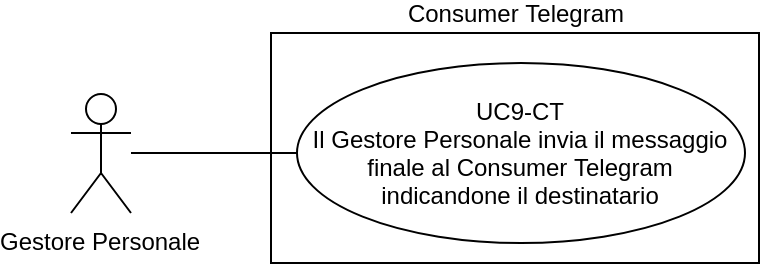
\includegraphics[width=0.6\textwidth]{img/casi_d'uso/UC9.png}\\
%		\caption{UC\theuccount-CT - Gestore Personale invia il messaggio finale al Consumer Telegram}
%	\end{figure}
	\begin{itemize}
		\item \textbf{Codice}: UC\theuccount-CT.
		\item \textbf{Titolo}: Gestore Personale invia il messaggio finale al Consumer Telegram.
		\item \textbf{Attori primari}: Gestore Personale.
		\item \textbf{Descrizione}: il Gestore Personale, dopo aver ricevuto il messaggio elaborato
		dal Producer Redmine o GitLab, controlla i Topic del messaggio, gli utenti iscritti, la loro disponibilità e se la loro preferenza è Telegram.
		Se tutte queste condizioni sono verificate, viene preparato il messaggio finale da inviare successivamente viene inviato al Consumer Telegram. 
		Se il destinatario è iscritto a quel Topic ma non è disponibile, il destinatario viene cambiato con la persona di fiducia. \par
		Il messaggio finale, una volta elaborato, conterrà i campi:
		\begin{itemize}
			\item Id della chat del destinatario
			\item Applicazione di provenienza
			\item Ora di invio
			\item Tipo di segnalazione(commit o issue)
			\item Project
			\item Topic
			\item Subject e opzionalmente
		 	\begin{itemize}
				\item Description
				\item Due date
				\item Milestone
				\item Assignee
			\end{itemize}
		\end{itemize}
		\item \textbf{Precondizione}: il Gestore Personale ha ricevuto il messaggio elaborato dal Producer Redmine o GitLab.
		\item \textbf{Postcondizione}: Il Gestore Personale ha inviato il messaggio finale al Consumer Telegram.
		\item \textbf{Scenario principale}: 
		\begin{enumerate}
			\item ll Gestore Personale riceve un messaggio dal Producer Redmine o dal Producer GitLab
			\item Il Gestore Personale valuta quali utenti sono iscritti al Topic del messaggio ricevuto e se vogliono ricevere il messaggio tramite Telegram
			\item Il Gestore Personale procede all'invio del messaggio finale al Consumer Telegram
		\end{enumerate}
		
	\end{itemize}

\stepcounter{uccount}
%\clearpage
\subsubsection{UC\theuccount-CE - Gestore Personale invia il messaggio finale al Consumer Email}
	\begin{figure}[H]
		\centering
		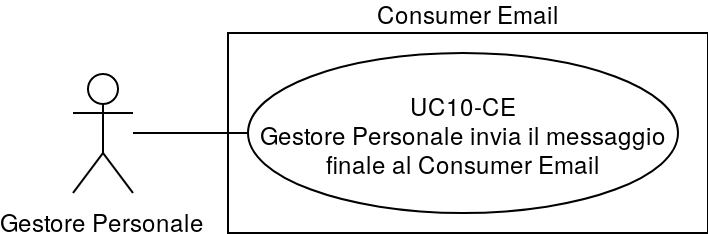
\includegraphics[width=0.6\textwidth]{img/casi_d'uso/UC10.png}\\
		\caption{UC\theuccount-CE - Gestore Personale invia il messaggio finale al Consumer Email}
	\end{figure}
	\begin{itemize}
		\item \textbf{Codice}: UC\theuccount-CE.
		\item \textbf{Titolo}: Gestore Personale invia il messaggio finale al Consumer Email.
		\item \textbf{Attori primari}: Gestore Personale.
		\item \textbf{Descrizione}: il Gestore Personale, dopo aver ricevuto il messaggio elaborato dai
		Producer Redmine o GitLab, controlla i messaggi sullo specifico Topic "commits", se ce ne sono
		vengono analizzati in base alla	lista di keyword. Se gli utenti iscritti a quella determinata
		keyword sono disponibili e se vogliono ricevere il messaggio tramite Email viene preparato il
		messaggio finale da inviare e inviato al Consumer Email. Altrimenti valuta il campo Topic del
		messaggio e controlla chi è iscritto a quel Topic, se gli utenti iscritti a quel Topic sono
		disponibili e se vogliono ricevere il messaggio tramite Email. Se tutte queste condizioni sono
		verificate, viene preparato il messaggio finale da inviare e inviato al Consumer Email.\\
		Il messaggio finale, una volta elaborato, conterrà i campi:
		\begin{itemize}
			\item Email del destinatario
			\item Applicazione di provenienza
			\item Ora di invio
			\item Tipo di segnalazione(commit, issue)
			\item Project
			\item Topic
			\item Subject e opzionalmente
		 	\begin{itemize}
				\item Description
				\item Due date
				\item Milestone
				\item Assignee
			\end{itemize}
		\end{itemize}
		\item \textbf{Precondizione}: il Gestore Personale ha ricevuto il messaggio elaborato dai Producer Redmine o GitLab.
		\item \textbf{Postcondizione}: Il Gestore Personale ha inviato il messaggio finale al Consumer Email.
		\item \textbf{Scenario principale}: 
		\begin{enumerate}
			\item ll Gestore Personale riceve un messaggio dal Producer Redmine o dal Producer GitLab
			\item Il Gestore Personale valuta quali utenti sono iscritti al Topic del messaggio ricevuto, se sono disponibili e se vogliono ricevere il messaggio tramite Email
			\item Gestore Personale procede all'invio del messaggio finale al Consumer Email
		\end{enumerate}
		
	\end{itemize}

\stepcounter{uccount}
%\clearpage
\subsubsection{UC\theuccount-GP - Inserimento utente}
		\begin{figure}[H]
			\centering
				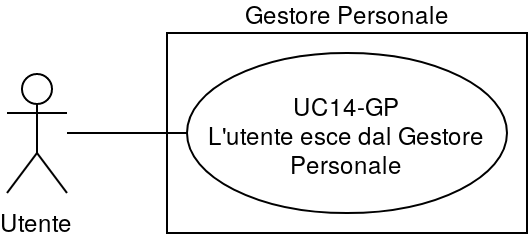
\includegraphics[width=\columnwidth]{img/casi_d'uso/UC14.png}\\
			\caption{UC\theuccount-GP - Inserimento utente}
		\end{figure}
	\begin{itemize}
		\item \textbf{Codice}: UC\theuccount-GP.
		\item \textbf{Titolo}: Inserimento utente.
		\item \textbf{Attori primari}: utente.
		\item \textbf{Descrizione}: l'utente, acceduto al sistema, aggiunge un nuovo utente nel sistema.
		Non è possibile che un utente non acceduto si iscriva da solo per la prima volta.
		In un primo momento è presente solo un utente predefinito che può aggiungere gli altri utenti.
		\item \textbf{Precondizione}: un nuovo utente deve essere aggiunto nel sistema.
		\item \textbf{Postcondizione}: un utente viene aggiunto al sistema.
		\item \textbf{Scenario principale}:
		\begin{enumerate}
			\item L'utente aggiunge un nuovo utente
		\end{enumerate}
	\end{itemize}
	%TODO:  aggiuora io, povero stronzo, che sono statonto.. come faccio a sapere qual è il mio identificativo?!
	\stepcounter{subuccount}
	\subsubsection{UC\theuccount.\thesubuccount-GP - Aggiunta nuovo utente}
		\begin{figure}[H]
			\centering
			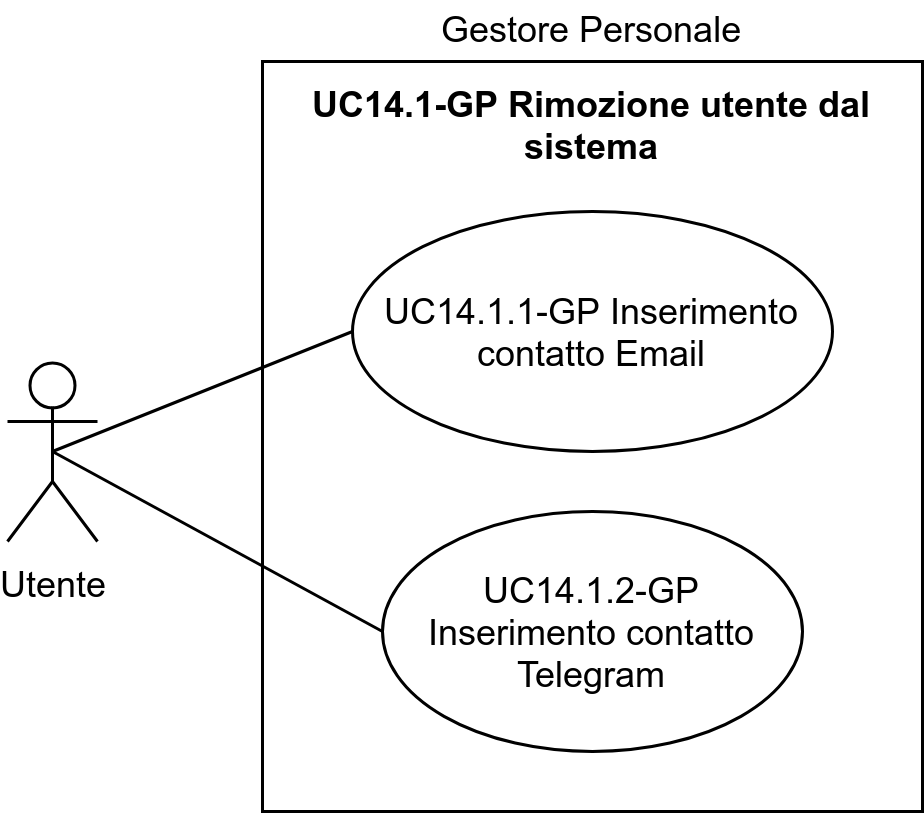
\includegraphics[width=\columnwidth]{img/casi_d'uso/UC14_1.png}\\
			\caption{UC\theuccount.\thesubuccount-GP - Aggiunta nuovo utente}
		\end{figure}
		\begin{itemize}
			\item \textbf{Codice}: C\theuccount.\thesubuccount-GP.
			\item \textbf{Titolo}: Aggiunta nuovo utente.
			\item \textbf{Attori primari}: utente.
			\item \textbf{Descrizione}: un nuovo utente viene inserito nel sistema.
			\item \textbf{Precondizione}: un nuovo utente deve essere aggiunto nel sistema.
			\item \textbf{Postcondizione}: un utente viene aggiunto al sistema.
			\item \textbf{Scenario principale}:
			\begin{enumerate}
				\item L'utente inserisce i dati del nuovo utente da aggiungere
				\item L'utente conferma l'invio dei dati
				\item L'aggiunta viene effettuata
			\end{enumerate}
			\item \textbf{Estensioni}:
			\begin{enumerate}
				\item Errore utente già presente nel sistema [UC\theuccount.2-GP]
			\end{enumerate}
		\end{itemize}

		\stepcounter{subsubuccount}
		\subsubsection{UC\theuccount.\thesubuccount.\thesubsubuccount-GP - Inserimento nome utente}

			\begin{itemize}
				\item \textbf{Codice}: UC\theuccount.\thesubuccount.\thesubsubuccount-GP.
				\item \textbf{Titolo}: inserimento nome utente.
				\item \textbf{Attori primari}: utente.
				%non registrato.
				\item \textbf{Descrizione}: l'utente inserisce il nominativo dell'utente da aggiungere.
				\item \textbf{Precondizione}: un nuovo utente deve essere aggiunto nel sistema.
				\item \textbf{Postcondizione}: il nome del nuovo utente è stato aggiunto nel sistema.
				\item \textbf{Scenario principale}:
				\begin{enumerate}
					\item L'utente aggiunge il nominativo del nuovo utente
				\end{enumerate}
			\end{itemize}

		\stepcounter{subsubuccount}
		\subsubsection{UC\theuccount.\thesubuccount.\thesubsubuccount-GP - Inserimento cognome utente}

			\begin{itemize}
				\item \textbf{Codice}: UC\theuccount.\thesubuccount.\thesubsubuccount-GP.
				\item \textbf{Titolo}: inserimento cognome utente.
				\item \textbf{Attori primari}: utente.
				% non registrato.
				\item \textbf{Descrizione}: l'utente inserisce il cognome dell'utente da aggiungere.
				\item \textbf{Precondizione}: un nuovo utente deve essere aggiunto nel sistema.
				\item \textbf{Postcondizione}: il cognome del nuovo utente è stato aggiunto nel sistema.
				\item \textbf{Scenario principale}:
				\begin{enumerate}
					\item L'utente aggiunge il cognome del nuovo utente
				\end{enumerate}
			\end{itemize}

		\stepcounter{subsubuccount}
		\subsubsection{UC\theuccount.\thesubuccount.\thesubsubuccount-GP - Inserimento contatto Email}

			\begin{itemize}
				\item \textbf{Codice}: UC\theuccount.\thesubuccount.\thesubsubuccount-GP.
				\item \textbf{Titolo}: inserimento contatto Email.
				\item \textbf{Attori primari}: utente.
				% non registrato.
				\item \textbf{Descrizione}: l'utente inserisce il contatto Email dell'utente da aggiungere.
				\item \textbf{Precondizione}: un nuovo utente deve essere aggiunto nel sistema.
				\item \textbf{Postcondizione}: il contatto Email è stato aggiunto.
				\item \textbf{Scenario principale}:
				\begin{enumerate}
					\item L'utente aggiunge il contatto Email del nuovo utente
				\end{enumerate}
		\end{itemize}

		\stepcounter{subsubuccount}
		\subsubsection{UC\theuccount.\thesubuccount.\thesubsubuccount-GP - Inserimento contatto Telegram}

			\begin{itemize}
				\item \textbf{Codice}: UC\theuccount.\thesubuccount.\thesubsubuccount-GP.
				\item \textbf{Titolo}: inserimento contatto Telegram.
				\item \textbf{Attori primari}: utente.
				% non registrato.
				\item \textbf{Descrizione}: l'utente inserisce il contatto Telegram dell'utente da aggiungere.
				\item \textbf{Precondizione}: un nuovo utente deve essere aggiunto nel sistema.
				\item \textbf{Postcondizione}: il contatto Telegram è stato aggiunto.
				\item \textbf{Scenario principale}:
				\begin{enumerate}
					\item L'utente aggiunge il contatto Telegram del nuovo utente
				\end{enumerate}
			\end{itemize}

	\stepcounter{subuccount}
	\subsubsection{UC\theuccount.\thesubuccount-GP - Errore utente già presente nel sistema}

		\begin{itemize}
			\item \textbf{Codice}: UC\theuccount.\thesubuccount-GP.
			\item \textbf{Titolo}: errore utente già presente nel sistema.
			\item \textbf{Attori primari}: utente.
			\item \textbf{Descrizione}: l’utente viene avvisato che i contatti Telegram o Email immessi non sono univoci.
			\item \textbf{Precondizione}: un nuovo utente deve essere aggiunto nel sistema.
			\item \textbf{Postcondizione}: il sistema comunica all’utilizzatore l’errore e l'utente non viene inserito.
			\item \textbf{Scenario principale}:
			\begin{enumerate}
				\item L'utente visualizza il messaggio d'errore
			\end{enumerate}
			\end{itemize}

\stepcounter{uccount}
%\clearpage
\subsubsection{UC\theuccount-GP - Rimozione utente}
		\begin{figure}[H]
			\centering
				\includegraphics[width=0.8\columnwidth]{img/casi_d'uso/UC\theuccount.png}\\
			\caption{UC\theuccount-GP - Rimozione utente}
		\end{figure}
	\begin{itemize}
		\item \textbf{Codice}: UC\theuccount-GP.
		\item \textbf{Titolo}: rimozione utente.
		\item \textbf{Attori primari}: utente.
		\item \textbf{Descrizione}: l'utente rimuove l'utente selezionato dal sistema.
		\item \textbf{Precondizione}: un utente già presente nel sistema deve essere rimosso.
		\item \textbf{Postcondizione}: un utente viene rimosso dal sistema.
		\item \textbf{Scenario principale}:
		\begin{enumerate}
			\item L'utente rimuove l'utente selezionato
		\end{enumerate}
\end{itemize}

	\stepcounter{subuccount}
	\subsubsection{UC\theuccount.\thesubuccount-GP - Rimozione utente dal sistema}
		\begin{figure}[H]
			\centering
			\includegraphics[width=0.5\columnwidth]{img/casi_d'uso/UC\theuccount_\thesubuccount.png}\\
			\caption{UC\theuccount.\thesubuccount-GP - Rimozione utente dal sistema}
		\end{figure}
		\begin{itemize}
			\item \textbf{Codice}: UC\theuccount.\thesubuccount-GP.
			\item \textbf{Titolo}: rimozione utente dal sistema.
			\item \textbf{Attori primari}: utente.
			\item \textbf{Descrizione}: un utente, acceduto al sistema, rimuove un utente presente nel sistema tramite l'inserimento del suo contatto Email o Telegram. Questo utente può essere anche se stesso.
			%il contatto Email o Telegram dell'utente da rimuovere è presente nel sistema, per cui la rimozione avviene con successo.
			\item \textbf{Precondizione}: un utente già presente nel sistema deve essere rimosso.
			\item \textbf{Postcondizione}: un utente con il contatto Email o Telegram inserito viene rimosso dal sistema.
			\item \textbf{Scenario principale}:
			\begin{enumerate}
				\item L'utente inserisce ciò che è richiesto dal sistema
				\item L'utente conferma l'invio dei dati
				\item L'utente da rimuovere è stato rimosso dal sistema
			\end{enumerate}
			\item \textbf{Estensioni}:
			\begin{itemize}
				\item Errore contatto non presente nel sistema [UC\theuccount.2-GP]
			\end{itemize}
		\end{itemize}

			\stepcounter{subsubuccount}
			\subsubsection{UC\theuccount.\thesubuccount.\thesubsubuccount-GP - Inserimento contatto Email}

				\begin{itemize}
					\item \textbf{Codice}: UC\theuccount.\thesubuccount.\thesubsubuccount-GP.
					\item \textbf{Titolo}: inserimento contatto Email.
					\item \textbf{Attori primari}: utente.
					\item \textbf{Descrizione}: l'utente ha aggiunto il contatto Email relativo all'utente che vuole rimuovere. L'inserimento di questo campo non avviene se viene invece inserito il contatto Telegram.
					\item \textbf{Precondizione}: un utente già presente nel sistema deve essere rimosso.
					\item \textbf{Postcondizione}: il contatto Email dell'utente da rimuovere è stato inserito.
					\item \textbf{Scenario principale}:
					\begin{enumerate}
						\item L'utente inserisce il contatto Email dell'utente da rimuovere
					\end{enumerate}
				\end{itemize}

			\stepcounter{subsubuccount}
			\subsubsection{UC\theuccount.\thesubuccount.\thesubsubuccount-GP - Inserimento contatto Telegram}

				\begin{itemize}
					\item \textbf{Codice}: UC\theuccount.\thesubuccount.\thesubsubuccount-GP.
					\item \textbf{Titolo}: inserimento contatto Telegram.
					\item \textbf{Attori primari}: utente.
					\item \textbf{Descrizione}: l'utente ha aggiunto il contatto Telegram relativo all'utente che vuole \newline rimuovere. L'inserimento di questo campo non avviene se viene invece inserito il contatto Email.
					\item \textbf{Precondizione}: un utente già presente nel sistema deve essere rimosso.
					\item \textbf{Postcondizione}: il contatto Telegram dell'utente da rimuovere è stato inserito.
					\item \textbf{Scenario principale}:
					\begin{enumerate}
						\item L'utente inserisce il contatto Telegram del utente da rimuovere.
					\end{enumerate}
				\end{itemize}

			\stepcounter{subuccount}
			\subsubsection{UC\theuccount.\thesubuccount-GP - Errore contatto non presente nel sistema}

				\begin{itemize}
					\item \textbf{Codice}: UC\theuccount.\thesubuccount-GP.
					\item \textbf{Titolo}: errore contatto non presente nel sistema.
					\item \textbf{Attori primari}: utente.
					\item \textbf{Descrizione}: l’utente viene avvisato che il contatto inserito non è presente nel sistema.
					\item \textbf{Precondizione}: un utente già presente nel sistema deve essere rimosso.
					\item \textbf{Postcondizione}: il sistema comunica all’utente che utilizza il sistema l’errore e nessun utente viene rimosso.
					\item \textbf{Scenario principale}:
					\begin{enumerate}
						\item L'utente selezionato attraverso il contatto Telegram o Email non viene rimosso perché non presente nel sistema.
					\end{enumerate}
				\end{itemize}


\stepcounter{uccount}
%\clearpage
\subsubsection{UC\theuccount-GP - Modifica utente}
		\begin{figure}[H]
			\centering
				\includegraphics[width=0.9\textwidth]{img/casi_d'uso/UC\theuccount.png}\\
			\caption{UC\theuccount-GP - Modifica utente}
		\end{figure}
	\begin{itemize}
		\item \textbf{Codice}: UC\theuccount-GP.
		\item \textbf{Titolo}: modifica utente.
		\item \textbf{Attori primari}: utente.
		\item \textbf{Descrizione}: l’utente vuole modificare le informazioni relative a un altro utente, o di se stesso.
		\item \textbf{Precondizione}: l'utente vuole modificare i dati di un utente già presente nel sistema.
		\item \textbf{Postcondizione}: i campi dell'utente sono stati modificati correttamente.
		\item \textbf{Scenario principale}:
		\begin{enumerate}
			\item L'utente modifica i dati relativi ad un utente
		\end{enumerate}
	\end{itemize}

	\stepcounter{subuccount}

		\subsubsection{UC\theuccount.\thesubuccount-GP - Modifica di un utente del sistema}
			\begin{figure}[H]
				\centering
				\includegraphics[width=0.6\columnwidth]{img/casi_d'uso/UC\theuccount_\thesubuccount.png}\\
				\caption{UC\theuccount.\thesubuccount-GP - Modifica di un utente del sistema}
			\end{figure}
			\begin{itemize}
				\item \textbf{Codice}: UC\theuccount.\thesubuccount-GP.
				\item \textbf{Titolo}: modifica di un utente del sistema.
				\item \textbf{Attori primari}: utente.
				\item \textbf{Descrizione}: l'identificativo è presente nel sistema e ne vengono modificati i relativi campi.
				\item \textbf{Precondizione}: l'utente vuole modificare un utente già presente nel sistema.
				\item \textbf{Postcondizione}: l'utente è stato modificato.
				\item \textbf{Scenario principale}:
				\begin{enumerate}
					\item L'utente viene modificato
				\end{enumerate}
				\item \textbf{Estensioni}:
				\begin{itemize}
					\item Errore, nuovi dati dell'utente già esistenti [UC\theuccount.2-GP]
				\end{itemize}
			\end{itemize}

			\stepcounter{subsubuccount}
			\subsubsection{UC\theuccount.\thesubuccount.\thesubsubuccount-GP - Inserimento del nuovo nome}
				\begin{itemize}
					\item \textbf{Codice}: UC\theuccount.\thesubuccount.\thesubsubuccount-GP.
					\item \textbf{Titolo}: inserimento del nuovo nome.
					\item \textbf{Attori primari}: utente.
					\item \textbf{Descrizione}: l'utente aggiunge il nuovo nome relativo all'identificativo inserito che vuole modificare.
					\item \textbf{Precondizione}: l'utente vuole modificare un utente già presente nel sistema.
					\item \textbf{Postcondizione}: il nome è stato inserito.
					\item \textbf{Scenario principale}:
					\begin{enumerate}
						\item L'utente inserisce il nuovo nome dell'utente che vuole modificare
					\end{enumerate}
				\end{itemize}

			\stepcounter{subsubuccount}

			\subsubsection{UC\theuccount.\thesubuccount.\thesubsubuccount-GP - Inserimento del nuovo cognome}
				\begin{itemize}
					\item \textbf{Codice}: UC\theuccount.\thesubuccount.\thesubsubuccount-GP.
					\item \textbf{Titolo}: inserimento del nuovo cognome.
					\item \textbf{Attori primari}: utente.
					\item \textbf{Descrizione}: l'utente aggiunge il nuovo cognome relativo all'identificativo inserito che vuole modificare.
					\item \textbf{Precondizione}: l'utente vuole modificare un utente già presente nel sistema.
					\item \textbf{Postcondizione}: il cognome è stato inserito.
					\item \textbf{Scenario principale}:
					\begin{enumerate}
						\item L'utente inserisce il nuovo cognome dell'utente che vuole modificare.
					\end{enumerate}
				\end{itemize}

			\stepcounter{subsubuccount}
			\subsubsection{UC\theuccount.\thesubuccount.\thesubsubuccount-GP - Inserimento del nuovo contatto Email}
				\begin{itemize}
					\item \textbf{Codice}: UC\theuccount.\thesubuccount.\thesubsubuccount-GP.
					\item \textbf{Titolo}: inserimento del nuovo contatto Email.
					\item \textbf{Attori primari}: utente.
					\item \textbf{Descrizione}: l'utente aggiunge il nuovo contatto Email relativo all'identificativo inserito che vuole modificare.
					\item \textbf{Precondizione}: l'utente vuole modificare un utente già presente nel sistema.
					\item \textbf{Postcondizione}: il contatto Email è stato inserito.
					\item \textbf{Scenario principale}:
					\begin{enumerate}
						\item L'utente inserisce il nuovo contatto Email dell'utente che vuole modificare
					\end{enumerate}
				\end{itemize}

			\stepcounter{subsubuccount}
			\subsubsection{UC\theuccount.\thesubuccount.\thesubsubuccount-GP - Inserimento del nuovo contatto Telegram}

				\begin{itemize}
					\item \textbf{Codice}: UC\theuccount.\thesubuccount.\thesubsubuccount-GP.
					\item \textbf{Titolo}: inserimento del nuovo contatto Telegram.
					\item \textbf{Attori primari}: utente.
					\item \textbf{Descrizione}: l'utente aggiunge il nuovo contatto Telegram relativo all'identificativo inserito che vuole modificare.
					\item \textbf{Precondizione}: l'utente vuole modificare un utente già presente nel sistema.
					\item \textbf{Postcondizione}: il contatto Telegram è stato inserito.
					\item \textbf{Scenario principale}:
					\begin{enumerate}
						\item L'utente inserisce il nuovo contatto Telegram dell'utente che vuole modificare
					\end{enumerate}
				\end{itemize}

		\stepcounter{subuccount}
		\subsubsection{UC\theuccount.\thesubuccount-GP - Errore, nuovi dati dell'utente già esistenti}

		\begin{itemize}
			\item \textbf{Codice}: UC\theuccount.\thesubuccount-GP.
			\item \textbf{Titolo}: errore, nuovi dati dell'utente già esistenti.
			\item \textbf{Attori primari}: utente.
			\item \textbf{Descrizione}: i nuovi dati dell'utente da modificare che sono stati inseriti sono già presenti nel sistema, ovvero i nuovi campi corrispondono a quelli di un utente già esistente. In particolare il contatto Telegram o Email, perchè una persona può avere lo stesso nome e cognome di un altro, ma non la stessa Email e nemmeno lo stesso identificativo Telegram.
			\item \textbf{Precondizione}: l'utente vuole modificare un utente già presente nel sistema.
			\item \textbf{Postcondizione}: l'utente non è stato modificato e viene visualizzato un messaggio di errore.
			\item \textbf{Scenario principale}:
			\begin{enumerate}
				\item L'utente inserisce i campi richiesti dal sistema per la modifica di un utente
				\item L'utente visualizza un messaggio di errore
			\end{enumerate}
		\end{itemize}

%	\stepcounter{subuccount}
%	\subsubsection{UC\theuccount.\thesubuccount-GP - Errore identificativo inesistente}
%
%		\begin{itemize}
%			\item \textbf{Codice}: UC\theuccount.\thesubuccount-GP.
%			\item \textbf{Titolo}: errore identificativo inesistente.
%			\item \textbf{Attori primari}: utente.
%			\item \textbf{Descrizione}:  l’utente inserisce l'identificativo dell'utente di cui vuole modificare le informazioni, ma viene avvisato che ha inserito un'identificativo errato perchè esso non è presente all'interno del sistema.
%			\item \textbf{Precondizione}: l'utente vuole modificare un utente già presente.
%			\item \textbf{Postcondizione}: il sistema comunica all’utilizzatore l’errore.
%			\item \textbf{Scenario principale}:
%			\begin{enumerate}
%				\item L'utente inserisce un identificativo errato
%				\item Il sistema comunica all’utilizzatore l’errore
%			\end{enumerate}
%		\end{itemize}


\stepcounter{uccount}
%\clearpage
\subsubsection{UC\theuccount-GP - Rimozione utente}
		\begin{figure}[H]
			\centering
				\includegraphics[width=\columnwidth]{img/casi_d'uso/UC\theuccount.png}\\
			\caption{UC\theuccount-GP - Rimozione utente}
		\end{figure}
	\begin{itemize}
		\item \textbf{Codice}: UC\theuccount-GP.
		\item \textbf{Titolo}: rimozione utente.
		\item \textbf{Attori primari}: utente.
		\item \textbf{Descrizione}: l'utente rimuove l'utente selezionato dal sistema.
		\item \textbf{Precondizione}: un utente già presente nel sistema deve essere rimosso.
		\item \textbf{Postcondizione}: un utente viene rimosso dal sistema.
		\item \textbf{Scenario principale}:
		\begin{enumerate}
			\item L'utente rimuove l'utente selezionato
		\end{enumerate}
\end{itemize}

	\stepcounter{subuccount}
	\subsubsection{UC\theuccount.\thesubuccount-GP - Rimozione utente dal sistema}
		\begin{figure}[H]
			\centering
			\includegraphics[width=0.6\columnwidth]{img/casi_d'uso/UC\theuccount_\thesubuccount.png}\\
			\caption{UC\theuccount.\thesubuccount-GP - Rimozione utente dal sistema}
		\end{figure}
		\begin{itemize}
			\item \textbf{Codice}: UC\theuccount.\thesubuccount-GP.
			\item \textbf{Titolo}: rimozione utente dal sistema.
			\item \textbf{Attori primari}: utente.
			\item \textbf{Descrizione}: un utente, acceduto al sistema, rimuove un utente presente nel sistema tramite l'inserimento del suo contatto Email o Telegram. Questo utente può essere anche se stesso.
			%il contatto Email o Telegram dell'utente da rimuovere è presente nel sistema, per cui la rimozione avviene con successo.
			\item \textbf{Precondizione}: un utente già presente nel sistema deve essere rimosso.
			\item \textbf{Postcondizione}: un utente con il contatto Email o Telegram inserito viene rimosso dal sistema.
			\item \textbf{Scenario principale}:
			\begin{enumerate}
				\item L'utente inserisce ciò che è richiesto dal sistema
				\item L'utente conferma l'invio dei dati
				\item L'utente da rimuovere è stato rimosso dal sistema
			\end{enumerate}
			\item \textbf{Estensioni}:
			\begin{itemize}
				\item Errore contatto non presente nel sistema [UC\theuccount.2-GP]
			\end{itemize}
		\end{itemize}

			\stepcounter{subsubuccount}
			\subsubsection{UC\theuccount.\thesubuccount.\thesubsubuccount-GP - Inserimento contatto Email}

				\begin{itemize}
					\item \textbf{Codice}: UC\theuccount.\thesubuccount.\thesubsubuccount-GP.
					\item \textbf{Titolo}: inserimento contatto Email.
					\item \textbf{Attori primari}: utente.
					\item \textbf{Descrizione}: l'utente ha aggiunto il contatto Email relativo all'utente che vuole rimuovere. L'inserimento di questo capo non avviene se viene invece inserito il contatto Telegram.
					\item \textbf{Precondizione}: un utente già presente nel sistema deve essere rimosso.
					\item \textbf{Postcondizione}: il contatto dell'utente da rimuovere Email è stato inserito.
					\item \textbf{Scenario principale}:
					\begin{enumerate}
						\item L'utente inserisce il contatto Email dell'utente da rimuovere
					\end{enumerate}
				\end{itemize}

			\stepcounter{subsubuccount}
			\subsubsection{UC\theuccount.\thesubuccount.\thesubsubuccount-GP - Inserimento contatto Telegram}

				\begin{itemize}
					\item \textbf{Codice}: UC\theuccount.\thesubuccount.\thesubsubuccount-GP.
					\item \textbf{Titolo}: inserimento contatto Telegram.
					\item \textbf{Attori primari}: utente.
					\item \textbf{Descrizione}: l'utente ha aggiunto il contatto Telegram relativo all'utente che vuole \newline rimuovere. L'inserimento di questo capo non avviene se viene invece inserito il contatto Email.
					\item \textbf{Precondizione}: un utente già presente nel sistema deve essere rimosso.
					\item \textbf{Postcondizione}: il contatto Telegram dell'utente da rimuovere è stato inserito.
					\item \textbf{Scenario principale}:
					\begin{enumerate}
						\item L'utente inserisce il contatto Telegram del utente da rimuovere.
					\end{enumerate}
				\end{itemize}

			\stepcounter{subuccount}
			\subsubsection{UC\theuccount.\thesubuccount-GP - Errore contatto non presente nel sistema}

				\begin{itemize}
					\item \textbf{Codice}: UC\theuccount.\thesubuccount-GP.
					\item \textbf{Titolo}: errore contatto non presente nel sistema.
					\item \textbf{Attori primari}: utente.
					\item \textbf{Descrizione}: l’utente viene avvisato che il contatto inserito non è presente nel sistema.
					\item \textbf{Precondizione}: un utente già presente nel sistema deve essere rimosso.
					\item \textbf{Postcondizione}: il sistema comunica all’utente che utilizza il sistema l’errore e nessun utente viene rimosso.
					\item \textbf{Scenario principale}:
					\begin{enumerate}
						\item L'utente selezionato attraverso il contatto Telegram o Email non viene rimosso perché non presente nel sistema.
					\end{enumerate}
				\end{itemize}


\stepcounter{uccount}
%\clearpage
\subsubsection{UC\theuccount-GP - Inserimento utente}
		\begin{figure}[H]
			\centering
				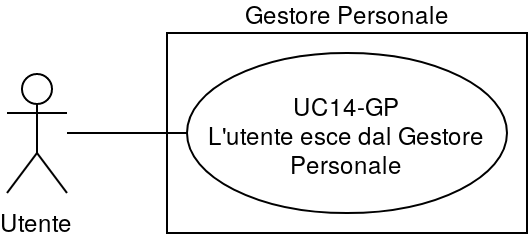
\includegraphics[width=\columnwidth]{img/casi_d'uso/UC14.png}\\
			\caption{UC\theuccount-GP - Inserimento utente}
		\end{figure}
	\begin{itemize}
		\item \textbf{Codice}: UC\theuccount-GP.
		\item \textbf{Titolo}: Inserimento utente.
		\item \textbf{Attori primari}: utente.
		\item \textbf{Descrizione}: l'utente, acceduto al sistema, aggiunge un nuovo utente nel sistema.
		Non è possibile che un utente non acceduto si iscriva da solo per la prima volta.
		In un primo momento è presente solo un utente predefinito che può aggiungere gli altri utenti.
		\item \textbf{Precondizione}: un nuovo utente deve essere aggiunto nel sistema.
		\item \textbf{Postcondizione}: un utente viene aggiunto al sistema.
		\item \textbf{Scenario principale}:
		\begin{enumerate}
			\item L'utente aggiunge un nuovo utente
		\end{enumerate}
	\end{itemize}
	%TODO:  aggiuora io, povero stronzo, che sono statonto.. come faccio a sapere qual è il mio identificativo?!
	\stepcounter{subuccount}
	\subsubsection{UC\theuccount.\thesubuccount-GP - Aggiunta nuovo utente}
		\begin{figure}[H]
			\centering
			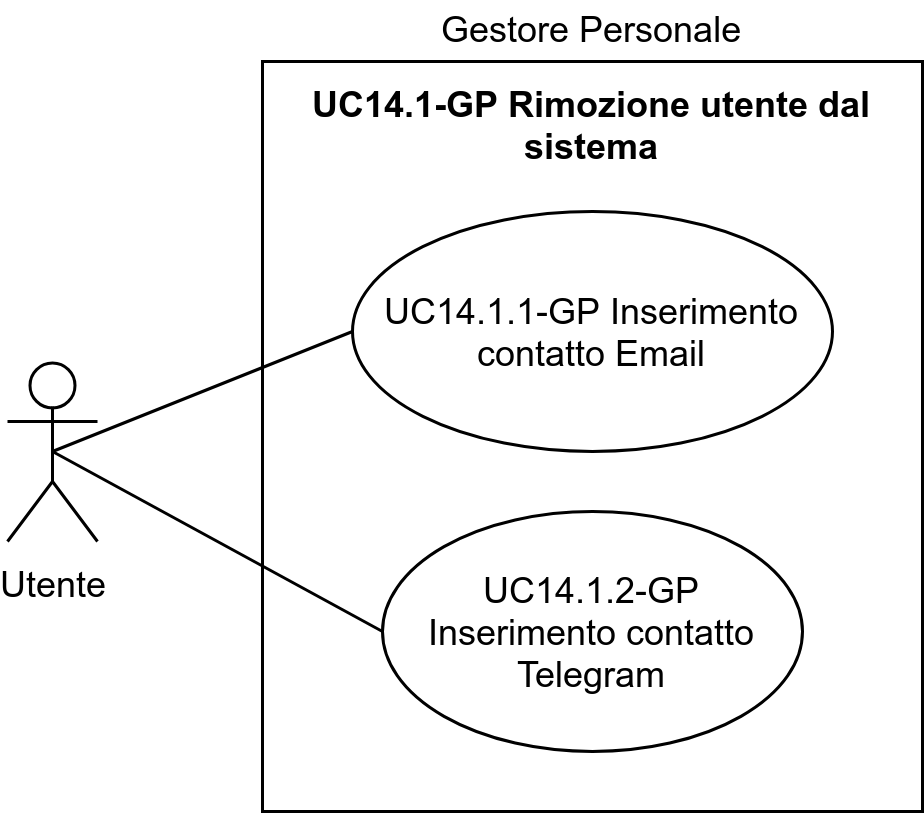
\includegraphics[width=\columnwidth]{img/casi_d'uso/UC14_1.png}\\
			\caption{UC\theuccount.\thesubuccount-GP - Aggiunta nuovo utente}
		\end{figure}
		\begin{itemize}
			\item \textbf{Codice}: C\theuccount.\thesubuccount-GP.
			\item \textbf{Titolo}: Aggiunta nuovo utente.
			\item \textbf{Attori primari}: utente.
			\item \textbf{Descrizione}: un nuovo utente viene inserito nel sistema.
			\item \textbf{Precondizione}: un nuovo utente deve essere aggiunto nel sistema.
			\item \textbf{Postcondizione}: un utente viene aggiunto al sistema.
			\item \textbf{Scenario principale}:
			\begin{enumerate}
				\item L'utente inserisce i dati del nuovo utente da aggiungere
				\item L'utente conferma l'invio dei dati
				\item L'aggiunta viene effettuata
			\end{enumerate}
			\item \textbf{Estensioni}:
			\begin{enumerate}
				\item Errore utente già presente nel sistema [UC\theuccount.2-GP]
			\end{enumerate}
		\end{itemize}

		\stepcounter{subsubuccount}
		\subsubsection{UC\theuccount.\thesubuccount.\thesubsubuccount-GP - Inserimento nome utente}

			\begin{itemize}
				\item \textbf{Codice}: UC\theuccount.\thesubuccount.\thesubsubuccount-GP.
				\item \textbf{Titolo}: inserimento nome utente.
				\item \textbf{Attori primari}: utente.
				%non registrato.
				\item \textbf{Descrizione}: l'utente inserisce il nominativo dell'utente da aggiungere.
				\item \textbf{Precondizione}: un nuovo utente deve essere aggiunto nel sistema.
				\item \textbf{Postcondizione}: il nome del nuovo utente è stato aggiunto nel sistema.
				\item \textbf{Scenario principale}:
				\begin{enumerate}
					\item L'utente aggiunge il nominativo del nuovo utente
				\end{enumerate}
			\end{itemize}

		\stepcounter{subsubuccount}
		\subsubsection{UC\theuccount.\thesubuccount.\thesubsubuccount-GP - Inserimento cognome utente}

			\begin{itemize}
				\item \textbf{Codice}: UC\theuccount.\thesubuccount.\thesubsubuccount-GP.
				\item \textbf{Titolo}: inserimento cognome utente.
				\item \textbf{Attori primari}: utente.
				% non registrato.
				\item \textbf{Descrizione}: l'utente inserisce il cognome dell'utente da aggiungere.
				\item \textbf{Precondizione}: un nuovo utente deve essere aggiunto nel sistema.
				\item \textbf{Postcondizione}: il cognome del nuovo utente è stato aggiunto nel sistema.
				\item \textbf{Scenario principale}:
				\begin{enumerate}
					\item L'utente aggiunge il cognome del nuovo utente
				\end{enumerate}
			\end{itemize}

		\stepcounter{subsubuccount}
		\subsubsection{UC\theuccount.\thesubuccount.\thesubsubuccount-GP - Inserimento contatto Email}

			\begin{itemize}
				\item \textbf{Codice}: UC\theuccount.\thesubuccount.\thesubsubuccount-GP.
				\item \textbf{Titolo}: inserimento contatto Email.
				\item \textbf{Attori primari}: utente.
				% non registrato.
				\item \textbf{Descrizione}: l'utente inserisce il contatto Email dell'utente da aggiungere.
				\item \textbf{Precondizione}: un nuovo utente deve essere aggiunto nel sistema.
				\item \textbf{Postcondizione}: il contatto Email è stato aggiunto.
				\item \textbf{Scenario principale}:
				\begin{enumerate}
					\item L'utente aggiunge il contatto Email del nuovo utente
				\end{enumerate}
		\end{itemize}

		\stepcounter{subsubuccount}
		\subsubsection{UC\theuccount.\thesubuccount.\thesubsubuccount-GP - Inserimento contatto Telegram}

			\begin{itemize}
				\item \textbf{Codice}: UC\theuccount.\thesubuccount.\thesubsubuccount-GP.
				\item \textbf{Titolo}: inserimento contatto Telegram.
				\item \textbf{Attori primari}: utente.
				% non registrato.
				\item \textbf{Descrizione}: l'utente inserisce il contatto Telegram dell'utente da aggiungere.
				\item \textbf{Precondizione}: un nuovo utente deve essere aggiunto nel sistema.
				\item \textbf{Postcondizione}: il contatto Telegram è stato aggiunto.
				\item \textbf{Scenario principale}:
				\begin{enumerate}
					\item L'utente aggiunge il contatto Telegram del nuovo utente
				\end{enumerate}
			\end{itemize}

	\stepcounter{subuccount}
	\subsubsection{UC\theuccount.\thesubuccount-GP - Errore utente già presente nel sistema}

		\begin{itemize}
			\item \textbf{Codice}: UC\theuccount.\thesubuccount-GP.
			\item \textbf{Titolo}: errore utente già presente nel sistema.
			\item \textbf{Attori primari}: utente.
			\item \textbf{Descrizione}: l’utente viene avvisato che i contatti Telegram o Email immessi non sono univoci.
			\item \textbf{Precondizione}: un nuovo utente deve essere aggiunto nel sistema.
			\item \textbf{Postcondizione}: il sistema comunica all’utilizzatore l’errore e l'utente non viene inserito.
			\item \textbf{Scenario principale}:
			\begin{enumerate}
				\item L'utente visualizza il messaggio d'errore
			\end{enumerate}
			\end{itemize}

\stepcounter{uccount}
%\clearpage
\subsubsection{UC\theuccount-GP - Rimozione preferenze}
		\begin{figure}[H]
			\centering
				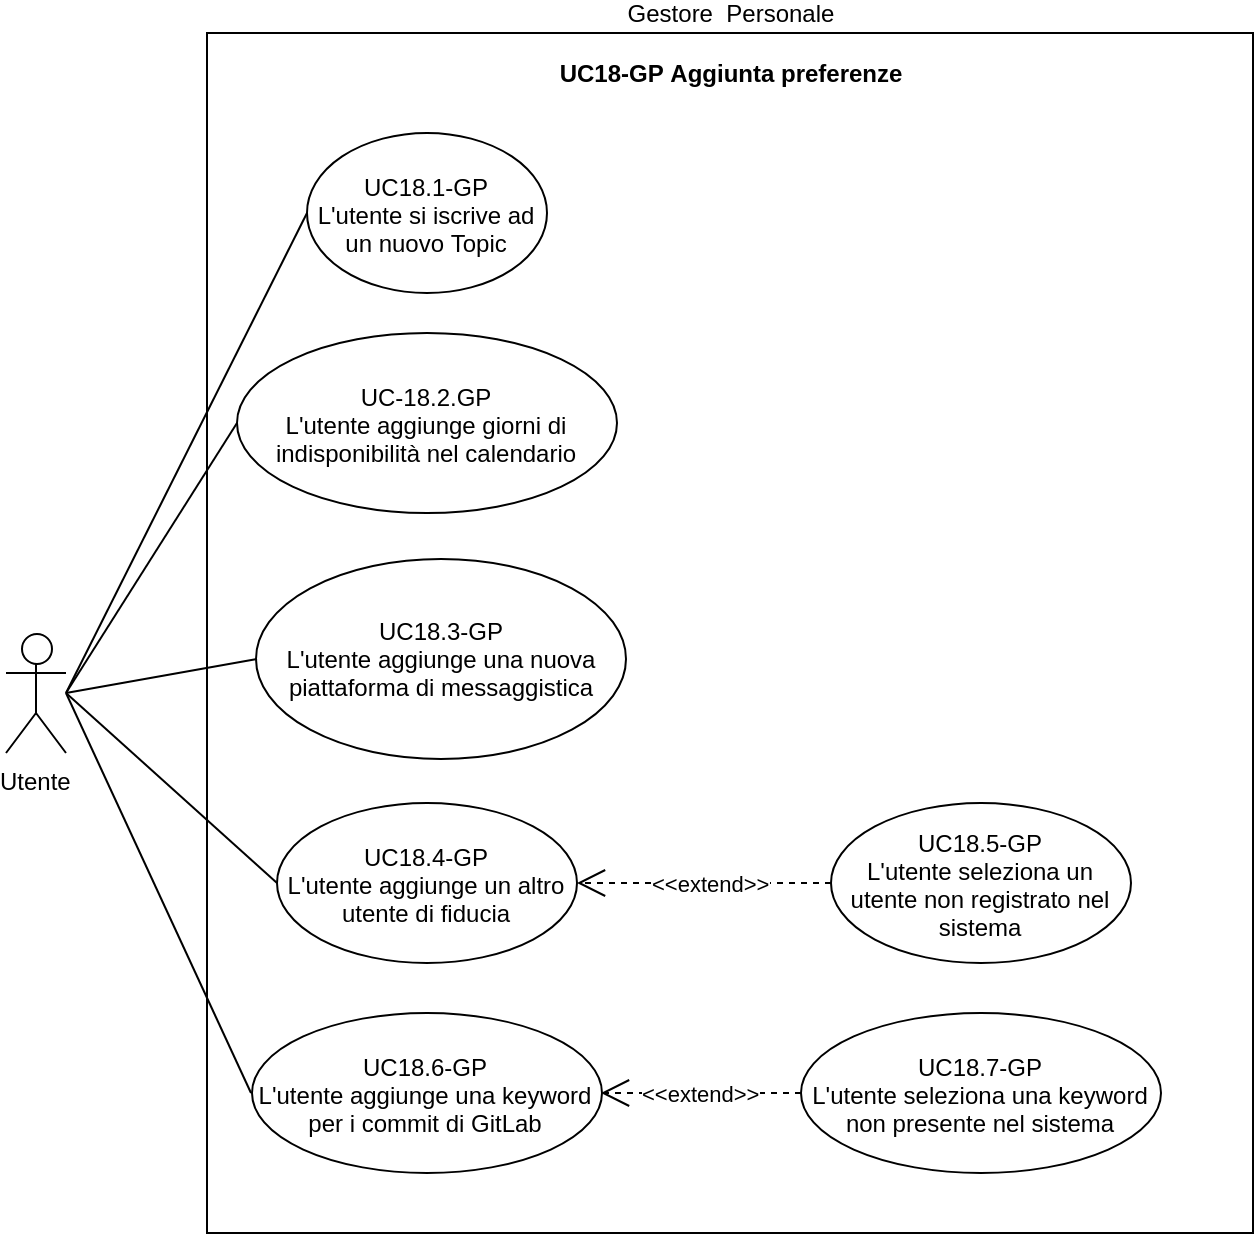
\includegraphics[width=\textwidth]{img/casi_d'uso/UC18.png}\\
			\caption{UC\theuccount-GP - Rimozione preferenze}
		\end{figure}
	\begin{itemize}
		\item \textbf{Codice}: UC\theuccount-GP.
		\item \textbf{Titolo}: rimozione preferenze.
		\item \textbf{Attori primari}: utente.
		\item \textbf{Descrizione}: l’utente, dopo aver selezionato delle preferenze dalle opzioni di configurazione, ne rimuove una o più. Le preferenze consistono in Topic, date di calendario e la piattaforma di messaggistica (Telegram e email).
		\item \textbf{Precondizione}: l’utente ha eseguito l'accesso nel sistema ed è presente almeno	una preferenza selezionata tra quelle proposte da Butterfly.
		\item \textbf{Postcondizione}: la nuova configurazione contiene una o più preferenze in meno rispetto	a quella precedente.
		\item \textbf{Scenario principale}:
		\begin{enumerate}
			\item L'utente procede alla rimozione di una o più preferenze
		\end{enumerate}
	\end{itemize}

	\stepcounter{subuccount}
	\subsubsection{UC\theuccount.\thesubuccount-GP - Disiscrizione Topic}

		\begin{itemize}
			\item \textbf{Codice}: UC\theuccount.\thesubuccount-GP.
			\item \textbf{Titolo}: disiscrizione Topic.
			\item \textbf{Attori primari}: utente.
			\item \textbf{Descrizione}: l’utente si disiscrive da uno o più Topic dai quali prima riceveva delle notifiche.
			\item \textbf{Precondizione}: l’utente ha acceduto correttamente nel sistema e non ha già selezionato tutti i Topic possibili proposti da \progetto.
			\item \textbf{Postcondizione}: il numero di Topic a cui è iscritto l’utente è diminuito.
			\item \textbf{Scenario principale}:
			\begin{enumerate}
				\item L'utente procede alla disiscrizione di uno o più Topic
			\end{enumerate}
		\end{itemize}

	\stepcounter{subuccount}
	\subsubsection{UC\theuccount.\thesubuccount-GP - Rimozione di uno o più giorni di irreperibilità nel calendario}

	\begin{itemize}
		\item \textbf{Codice}: UC\theuccount.\thesubuccount-GP.
		\item \textbf{Titolo}: rimozione di uno o più giorni di irreperibilità nel calendario.
		\item \textbf{Attori primari}: utente.
		\item \textbf{Descrizione}: l’utente rimuove i giorni di calendario in cui precedentemente	non era reperibile, tornando disponibile.
		\item \textbf{Precondizione}: l’utente ha acceduto correttamente nel sistema ed è presente almeno un giorno di calendario selezionato.
		\item \textbf{Postcondizione}: il numero di giorni di calendario in cui l’utente non è reperibile è diminuito.
		\item \textbf{Scenario principale}:
		\begin{enumerate}
			\item L'utente procede alla rimozione di uno o più giorni di irreperibilità
		\end{enumerate}
	\end{itemize}

	\stepcounter{subuccount}
	\subsubsection{UC\theuccount.\thesubuccount-GP - Rimozione preferenza piattaforma di messaggistica}

	\begin{itemize}
		\item \textbf{Codice}: UC\theuccount.\thesubuccount-GP.
		\item \textbf{Titolo}: rimozione preferenza piattaforma di messaggistica.
		\item \textbf{Attori primari}: utente.
		\item \textbf{Descrizione}: l’utente rimuove una o più preferenze tra Telegram e Email dalle	quali non vuole più ricevere notifiche tramite \progetto.
		\item \textbf{Precondizione}: l’utente ha acceduto correttamente nel sistema ed è presente almeno una piattaforma di messaggistica selezionata tra quelle proposte da \progetto.
		\item \textbf{Postcondizione}: il numero di piattaforme di messaggistica da cui l’utente vuole ricevere notifiche è diminuito.
		\item \textbf{Scenario principale}:
		\begin{enumerate}
			\item L'utente procede alla rimozione di una o più piattaforme di messaggistica
		\end{enumerate}
	\end{itemize}

	% \stepcounter{subuccount}
	% \subsubsection{UC\theuccount.\thesubuccount-GP - Rimozione persona di fiducia}

	% \begin{itemize}
	% 	\item \textbf{Codice}: UC\theuccount.\thesubuccount-GP.
	% 	\item \textbf{Titolo}: aggiunta persona di fiducia.
	% 	\item \textbf{Attori primari}: utente.
	% 	\item \textbf{Descrizione}:  l’utente rimuove l'utente legato a un identificativo di sua preferenza a cui inoltrare i messaggi in caso di indisponibilità.
	% 	\item \textbf{Precondizione}: l’utente ha eseguito l'accesso nel sistema e vuole rimuovere la sua persona di fiducia.
	% 	\item \textbf{Postcondizione}: la preferenza viene rimossa correttamente.
	% 	\item \textbf{Scenario principale}:
	% 	\begin{enumerate}
	% 		\item L’utente procede alla rimozione della sua persona di fiducia
	% 	\end{enumerate}
	% 	\item \textbf{Estensioni}:
	% 	\begin{enumerate}
	% 		\item Errore identificativo persona di fiducia inesistente [UC\theuccount.5-GP].
	% 	\end{enumerate}
	% \end{itemize}

	% \stepcounter{subuccount}
	% \subsubsection{UC\theuccount.\thesubuccount-GP - Errore identificativo persona di fiducia inesistente}

	% \begin{itemize}
	% 	\item \textbf{Codice}: UC\theuccount.\thesubuccount-GP.
	% 	\item \textbf{Titolo}: errore identificativo persona di fiducia inesistente.
	% 	\item \textbf{Attori primari}: utente.
	% 	\item \textbf{Descrizione}: l’utente viene avvisato che ha inserito un identificativo errato.
	% 	\item \textbf{Precondizione}: l’utente ha acceduto con le sue credenziali corrette nel sistema e vuole rimuovere la sua persona di fiducia.
	% 	\item \textbf{Postcondizione}: il sistema comunica all’utilizzatore l’errore.
	% 	\item \textbf{Scenario principale}:
	% 	\begin{enumerate}
	% 		\item L'utente inserisce l'identificativo della sua persona di fiducia
	% 		\item Il sistema rileva che questo identificativo non esiste
	% 		\item L'utente visualizza il messaggio di errore
	% 	\end{enumerate}
	% \end{itemize}

	\stepcounter{subuccount}
	\subsubsection{UC\theuccount.\thesubuccount-GP - Rimozione di keyword per i push di GitLab}

	\begin{itemize}
		\item \textbf{Codice}: UC\theuccount.\thesubuccount-GP.
		\item \textbf{Titolo}: rimozione di keyword per i push di GitLab.
		\item \textbf{Attori primari}: utente.
		\item \textbf{Descrizione}: l’utente seleziona e rimuove una o più keyword già presente nel sistema per non ricevere la notifica di push in
		cui i messaggi di commit contengono la keyword rimossa.
		\item \textbf{Precondizione}:  l’utente ha acceduto al sistema.
		\item \textbf{Postcondizione}: nelle nuove configurazioni dell'utente selezionato sono state rimosse delle keyword precedentemente presenti.
		\item \textbf{Scenario principale}:
		\begin{enumerate}
			\item L'utente rimuove una o più keyword per cui non vuole iù ricevere messaggi di push
		\end{enumerate}
		\item \textbf{Estensioni}:
		\begin{enumerate}
			\item Errore keyword da rimuovere non presente [UC\theuccount.7-GP]
		\end{enumerate}
	\end{itemize}

	\stepcounter{subuccount}
	\subsubsection{UC\theuccount.\thesubuccount-GP - Errore keyword da rimuovere non presente}

	\begin{itemize}
		\item \textbf{Codice}: UC\theuccount.\thesubuccount-GP.
		\item \textbf{Titolo}: errore keyword da rimuovere non presente.
		\item \textbf{Attori primari}: utente.
		\item \textbf{Descrizione}: l'utente vuole rimuovere una keyword che non ha mai inserito o che ha rimosso precedentemente.
		\item \textbf{Precondizione}: l’utente ha acceduto al sistema.
		\item \textbf{Postcondizione}: viene visualizzato un messaggio d'errore con indicato che la keyword	selezionata che non è presente nel sistema.
		\item \textbf{Scenario principale}:
		\begin{enumerate}
			\item L'utente inserisce la keyword che vuole rimuovere
			\item Il sistema rileva che non è presente
			\item L'utente visualizza il messaggio di errore
		\end{enumerate}
	\end{itemize}


\stepcounter{uccount}
%\clearpage
\subsubsection{UC\theuccount-GP - Modifica utente}
		\begin{figure}[H]
			\centering
				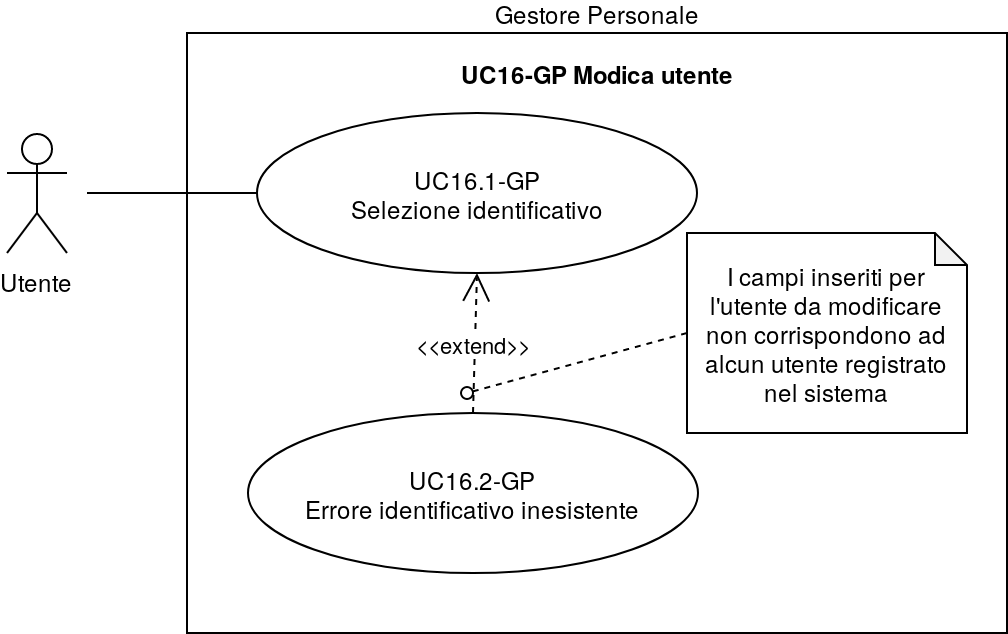
\includegraphics[width=0.8\textwidth]{img/casi_d'uso/UC16.png}\\
			\caption{UC\theuccount-GP - Modifica utente}
		\end{figure}
	\begin{itemize}
		\item \textbf{Codice}: UC\theuccount-GP.
		\item \textbf{Titolo}: modifica utente.
		\item \textbf{Attori primari}: utente.
		\item \textbf{Descrizione}: l’utente vuole modificare le informazioni relative a un altro utente, o di se stesso.
		\item \textbf{Precondizione}: l'utente vuole modificare i dati di un utente già presente nel sistema.
		\item \textbf{Postcondizione}: i campi dell'utente sono stati modificati correttamente.
		\item \textbf{Scenario Principale}:
		\begin{enumerate}
			\item L'utente modifica i dati relativi di un utente
		\end{enumerate}
	\end{itemize}
	
	\stepcounter{subuccount}
	\subsubsection{UC\theuccount.\thesubuccount-GP - Selezione identificativo}
		\begin{figure}[H]
			\centering
			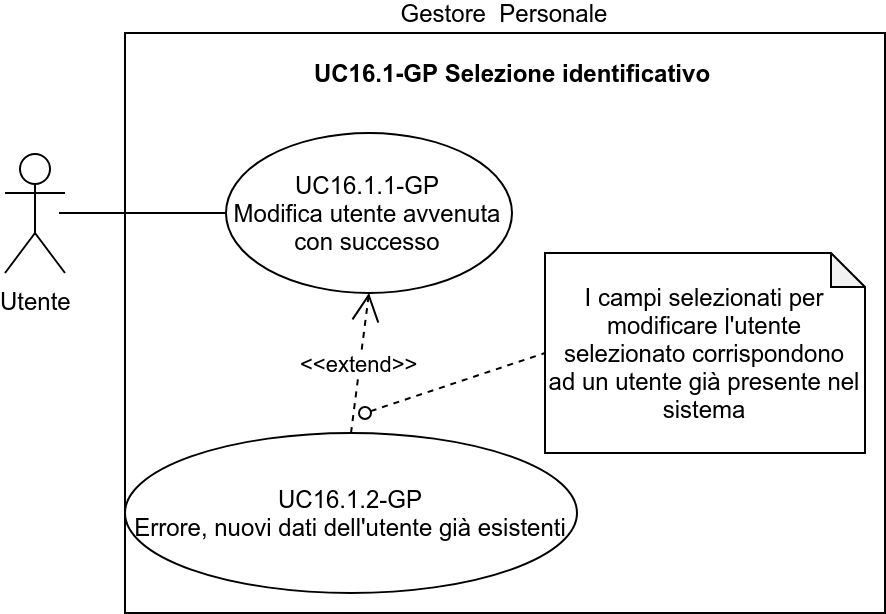
\includegraphics[width=0.8\textwidth]{img/casi_d'uso/UC16_1.png}\\
			\caption{UC\theuccount.\thesubuccount-GP - Selezione identificativo}
		\end{figure}
		\begin{itemize}
			\item \textbf{Codice}: UC\theuccount.\thesubuccount-GP.
			\item \textbf{Titolo}: selezione identificativo.
			\item \textbf{Attori primari}: utente.
			\item \textbf{Descrizione}: l'utente aggiunge l'identificativo dell'utente che vuole modificare.
			\item \textbf{Precondizione}: l'utente vuole modificare un utente già presente.
			\item \textbf{Postcondizione}: l'identificativo è stato inserito.
			\item \textbf{Scenario Principale}:
			\begin{enumerate}
				\item L'utente procede con l'inserimento dell'identificativo dell'utente da modificare
			\end{enumerate}
			\item \textbf{Estensioni}:
			\begin{itemize}
				\item Errore identificativo inesistente [UC\theuccount.2-GP]
			\end{itemize}
		\end{itemize}
		
		\stepcounter{subsubuccount}
		\subsubsection{UC\theuccount.\thesubuccount.\thesubsubuccount-GP - Modifica utente avvenuta con successo}
			\begin{figure}[H]
				\centering
				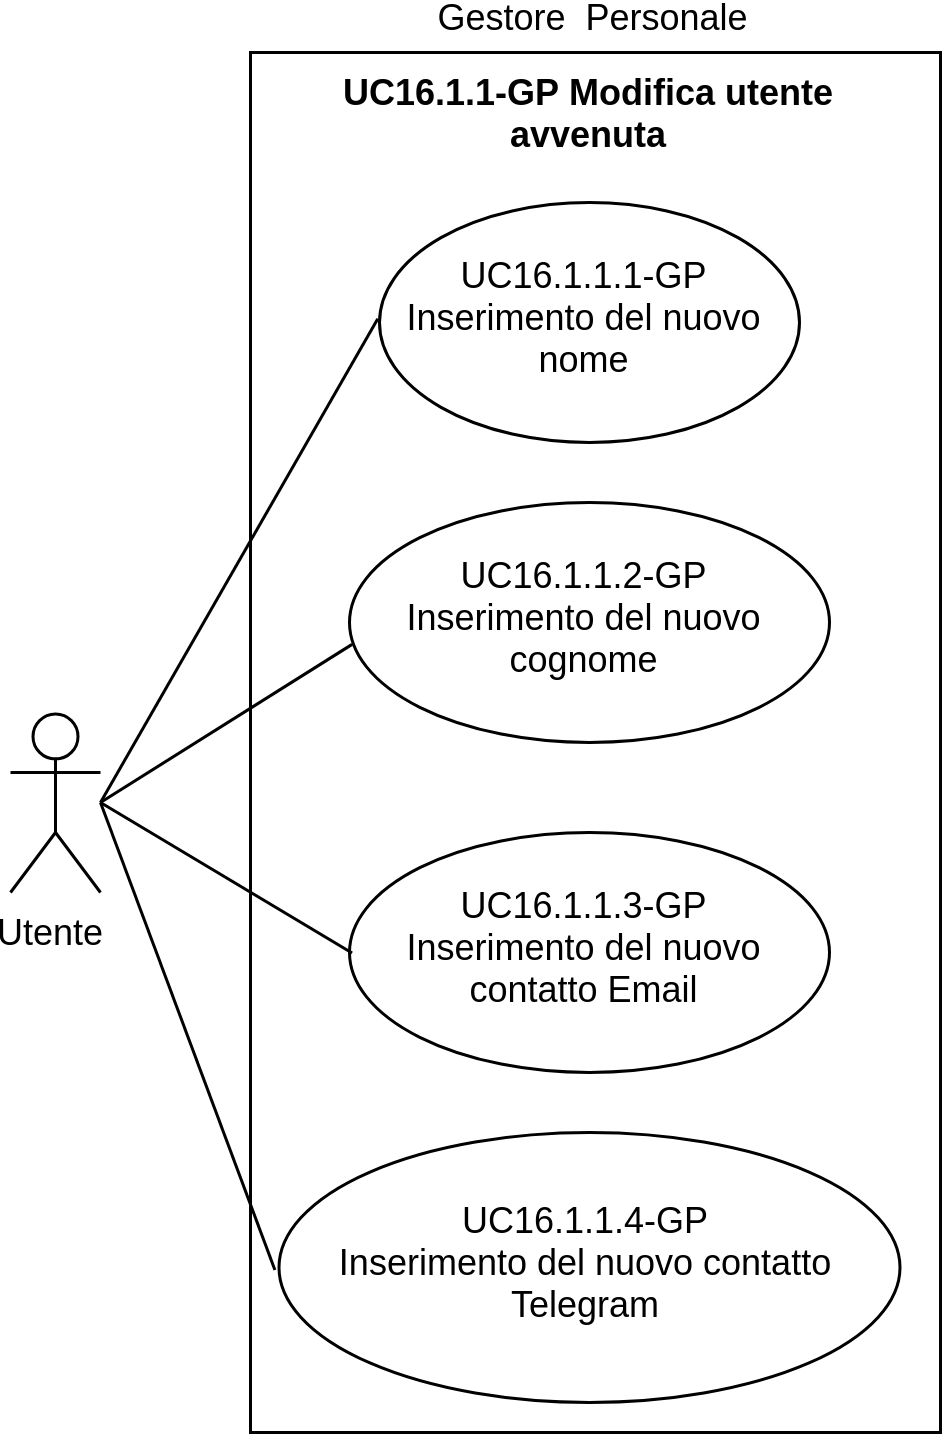
\includegraphics[width=0.5\columnwidth]{img/casi_d'uso/UC16_1_1.png}\\
				\caption{UC\theuccount.\thesubuccount.\thesubsubuccount-GP - Modifica utente avvenuta con successo}
			\end{figure}
			\begin{itemize}
				\item \textbf{Codice}: UC\theuccount.\thesubuccount.\thesubsubuccount-GP.
				\item \textbf{Titolo}: modifica utente avvenuta con successo.
				\item \textbf{Attori primari}: utente.
				\item \textbf{Descrizione}: l'identificativo è presente nel sistema e ne vengono modificati i relativi campi con successo.
				\item \textbf{Precondizione}: l'utente vuole modificare un utente già presente.
				\item \textbf{Postcondizione}: l'utente è stato modificato con successo.
				\item \textbf{Scenario Principale}:
				\begin{enumerate}
					\item L'utente viene modificato con successo
				\end{enumerate}
				\item \textbf{Estensioni}:
				\begin{itemize}
					\item Errore, nuovi dati dell'utente già esistenti [UC\theuccount.\thesubuccount.2-GP]
				\end{itemize}
			\end{itemize}
			
			\stepcounter{subsubsubuccount}
			\subsubsection{UC\theuccount.\thesubuccount.\thesubsubuccount.\thesubsubsubuccount-GP - Inserimento del nuovo nome}
				
				\begin{itemize}
					\item \textbf{Codice}: UC\theuccount.\thesubuccount.\thesubsubuccount.\thesubsubsubuccount-GP.
					\item \textbf{Titolo}: inserimento del nuovo nome.
					\item \textbf{Attori primari}: utente.
					\item \textbf{Descrizione}: l'utente aggiunge il nuovo nome relativo all'identificativo inserito che vuole modificare.
					\item \textbf{Precondizione}: l'utente vuole modificare un utente già presente.
					\item \textbf{Postcondizione}: il nome è stato inserito.
					\item \textbf{Scenario Principale}:
					\begin{enumerate}
						\item L'utente inserisce il nuovo nome dell'utente che vuole modificare
					\end{enumerate}
				\end{itemize}
			
			\stepcounter{subsubsubuccount}
			\subsubsection{UC\theuccount.\thesubuccount.\thesubsubuccount.\thesubsubsubuccount-GP - Inserimento del nuovo cognome}
				
				\begin{itemize}
					\item \textbf{Codice}: UC\theuccount.\thesubuccount.\thesubsubuccount.\thesubsubsubuccount-GP.
					\item \textbf{Titolo}: inserimento del nuovo cognome.
					\item \textbf{Attori primari}: utente.
					\item \textbf{Descrizione}: l'utente aggiunge il nuovo cognome relativo all'identificativo inserito che vuole modificare.
					\item \textbf{Precondizione}: l'utente vuole modificare un utente già presente.
					\item \textbf{Postcondizione}: il cognome è stato inserito.
					\item \textbf{Scenario Principale}:
					\begin{enumerate}
						\item L'utente inserisce il nuovo cognome dell'utente che vuole modificare.
					\end{enumerate}
				\end{itemize}
			
			\stepcounter{subsubsubuccount}
			\subsubsection{UC\theuccount.\thesubuccount.\thesubsubuccount.\thesubsubsubuccount-GP - Inserimento del nuovo contatto Email}
				
				\begin{itemize}
					\item \textbf{Codice}: UC\theuccount.\thesubuccount.\thesubsubuccount.\thesubsubsubuccount-GP.
					\item \textbf{Titolo}: inserimento del nuovo contatto Email.
					\item \textbf{Attori primari}: utente.
					\item \textbf{Descrizione}: l'utente aggiunge il nuovo contatto Email relativo all'identificativo inserito che vuole modificare.
					\item \textbf{Precondizione}: l'utente vuole modificare un utente già presente.
					\item \textbf{Postcondizione}: il contatto Email è stato inserito.
					\item \textbf{Scenario Principale}:
					\begin{enumerate}
						\item L'utente inserisce il nuovo contatto Email dell'utente che vuole modificare
					\end{enumerate}
				\end{itemize}
			
			\stepcounter{subsubsubuccount}
			\subsubsection{UC\theuccount.\thesubuccount.\thesubsubuccount.\thesubsubsubuccount-GP - Inserimento del nuovo contatto Telegram}
				
				\begin{itemize}
					\item \textbf{Codice}: UC\theuccount.\thesubuccount.\thesubsubuccount.\thesubsubsubuccount-GP.
					\item \textbf{Titolo}: inserimento del nuovo contatto Telegram.
					\item \textbf{Attori primari}: utente.
					\item \textbf{Descrizione}: l'utente aggiunge il nuovo contatto Telegram relativo all'identificativo inserito che vuole modificare.
					\item \textbf{Precondizione}: l'utente vuole modificare un utente già presente.
					\item \textbf{Postcondizione}: il contatto Telegram è stato inserito.
					\item \textbf{Scenario Principale}:
					\begin{enumerate}
						\item L'utente inserisce il nuovo contatto Telegram dell'utente che vuole modificare
					\end{enumerate}
				\end{itemize}
			
		\stepcounter{subsubuccount}
		\subsubsection{UC\theuccount.\thesubuccount.\thesubsubuccount-GP - Errore, nuovi dati dell'utente già esistenti}
		
		\begin{itemize}
			\item \textbf{Codice}: UC\theuccount.\thesubuccount.\thesubsubuccount-GP.
			\item \textbf{Titolo}: errore, nuovi dati dell'utente già esistenti.
			\item \textbf{Attori primari}: utente.
			\item \textbf{Descrizione}: i nuovi dati dell'utente da modificare che sono stati inseriti sono già presenti nel sistema.
			\item \textbf{Precondizione}: l'utente vuole modificare un utente già presente.
			\item \textbf{Postcondizione}: l'utente non è stato modificato.
			\item \textbf{Scenario Principale}:
			\begin{enumerate}
				\item L'utente non viene modificato perché i nuovi campi corrispondono a quelli di un utente già esistente
			\end{enumerate}
		\end{itemize}
	\stepcounter{subuccount}
	\subsubsection{UC\theuccount.\thesubuccount-GP - Errore identificativo inesistente}
		
		\begin{itemize}
			\item \textbf{Codice}: UC\theuccount.\thesubuccount-GP.
			\item \textbf{Titolo}: errore identificativo inesistente.
			\item \textbf{Attori primari}: utente.
			\item \textbf{Descrizione}:  l’utente viene avvisato che ha inserito un'identificativo errato.
			\item \textbf{Precondizione}: l'utente vuole modificare un utente già presente.
			\item \textbf{Postcondizione}: il sistema comunica all’utilizzatore l’errore.
			\item \textbf{Scenario Principale}:
			\begin{enumerate}
				\item L'utente ha inserito un identificativo errato e il sistema comunica all’utilizzatore l’errore.
			\end{enumerate}
		\end{itemize}

\stepcounter{uccount}
%\clearpage
\subsubsection{UC\theuccount-GP - Aggiunta preferenze}
		\begin{figure}[H]
			\centering
				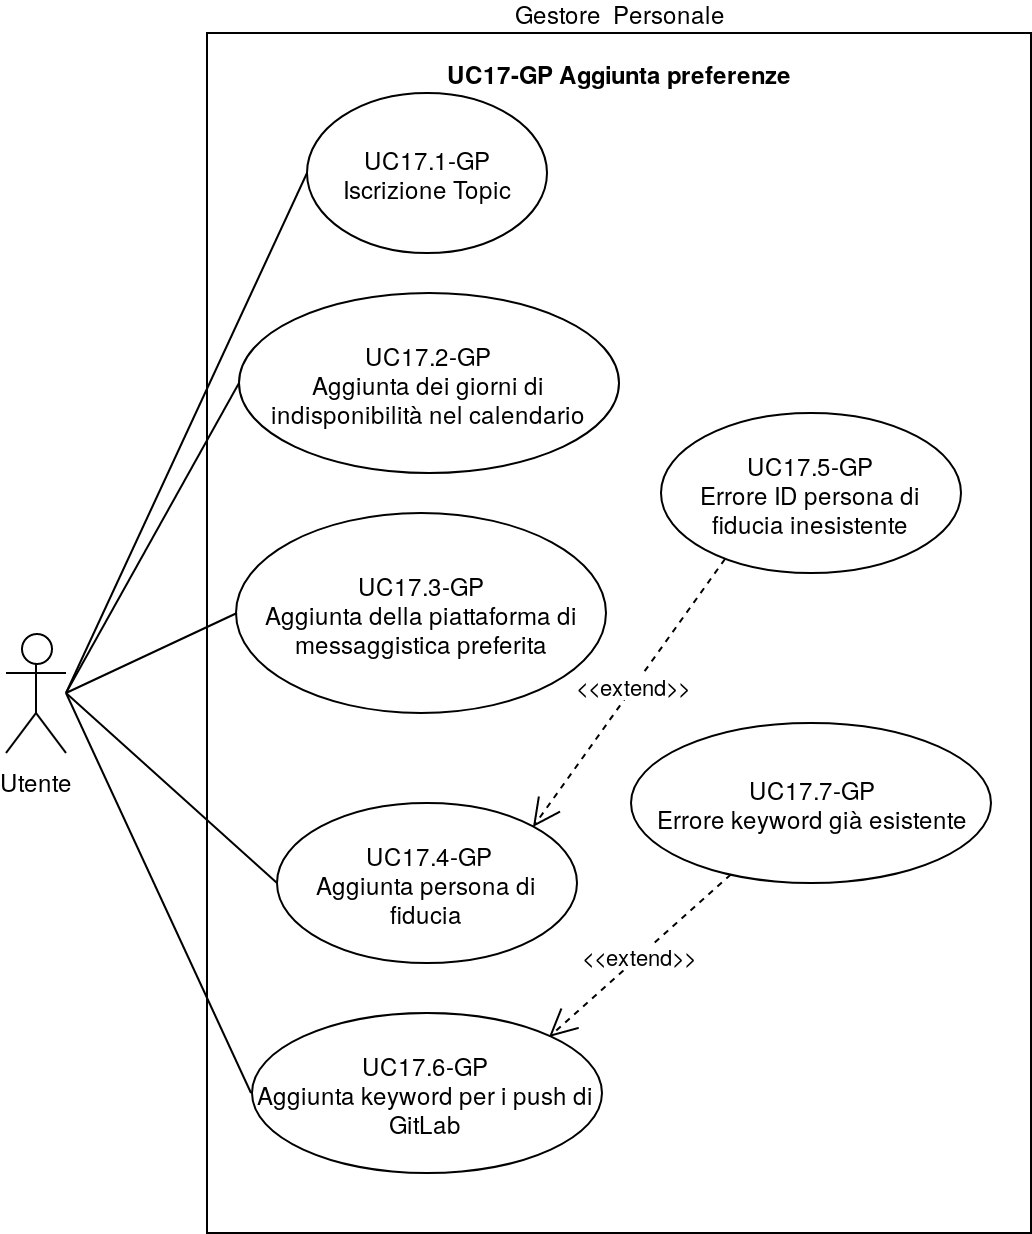
\includegraphics[width=1\textwidth]{img/casi_d'uso/UC17.png}\\
			\caption{UC\theuccount-GP - Aggiunta preferenze}
		\end{figure}
	\begin{itemize}
		\item \textbf{Codice}: UC\theuccount-GP.
		\item \textbf{Titolo}: aggiunta preferenze.
		\item \textbf{Attori primari}: utente.
		\item \textbf{Descrizione}: l’utente, date le varie opzioni per configurare Butterfly, aggiunge una
		preferenza tra Topic, giorni di calendario, piattaforma di messaggistica (Telegram o Email)	preferita e la persona di fiducia che lo può sostituire.
		\item \textbf{Precondizione}: l’utente ha acceduto con le sue credenziali corrette nel sistema e non ha già selezionato tutte le preferenze possibili proposte da \progetto.
		\item \textbf{Postcondizione}: la nuova configurazione contiene una o più preferenze in aggiunta rispetto a quella precedente.
		\item \textbf{Scenario principale}:
		\begin{enumerate}
			\item L'utente aggiunge una o più preferenze
		\end{enumerate}
	\end{itemize}

	\stepcounter{subuccount}
	\subsubsection{UC\theuccount.\thesubuccount-GP - Iscrizione Topic}

		\begin{itemize}
			\item \textbf{Codice}: UC\theuccount.\thesubuccount-GP.
			\item \textbf{Titolo}: iscrizione Topic.
			\item \textbf{Attori primari}: utente.
			\item \textbf{Descrizione}: data la lista di Topic presenti, l’utente ne seleziona uno o	più a cui è interessato, ricevendone una notifica. I Topic sono divisi per categoria e	comprendono etichette, progetto a cui sono legate e l'applicazione di provenienza: Redmine o GitLab.
			\item \textbf{Precondizione}: l’utente ha acceduto correttamente nel sistema e non ha già selezionato tutti i Topic possibili proposti da \progetto.
			\item \textbf{Postcondizione}: il numero di Topic a cui è interessato l’utente è aumentato.
			\item \textbf{Scenario principale}:
			\begin{enumerate}
				\item L'utente procede all'iscrizione di uno o più Topic
			\end{enumerate}
		\end{itemize}
	
	\stepcounter{subuccount}
	\subsubsection{UC\theuccount.\thesubuccount-GP - Aggiunta dei giorni di indisponibilità nel calendario}
		
		\begin{itemize}
			\item \textbf{Codice}: UC\theuccount.\thesubuccount-GP.
			\item \textbf{Titolo}: aggiunta dei giorni di indisponibilità nel calendario.
			\item \textbf{Attori primari}: utente.
			\item \textbf{Descrizione}: dato il calendario lavorativo, l’utente aggiunge uno o più giorni in cui non è reperibile e non vuole ricevere notifiche.
			\item \textbf{Precondizione}: l’utente ha acceduto correttamente nel sistema e vuole selezionare alcuni giorni di indisponibilità.
			\item \textbf{Postcondizione}: il numero di giorni in cui l’utente non si rende disponibile è aumentato.
			\item \textbf{Scenario principale}:
			\begin{enumerate}
				\item L'utente procede all'inserimento di uno o più giorni di indisponibilità
			\end{enumerate}
		\end{itemize}
	
	\stepcounter{subuccount}
	\subsubsection{UC\theuccount.\thesubuccount-GP - Aggiunta della piattaforma di messaggistica preferita}
		
		\begin{itemize}
			\item \textbf{Codice}: UC\theuccount.\thesubuccount-GP.
			\item \textbf{Titolo}: aggiunta della piattaforma di messaggistica preferita.
			\item \textbf{Attori primari}: utente.
			\item \textbf{Descrizione}: l’utente aggiunge la sua preferenza tra Telegram e Email dove vuole ricevere le notifiche.
			\item \textbf{Precondizione}: l’utente ha acceduto correttamente nel sistema e non ha già selezionato tutte le piattaforme di messaggistica possibili proposte da \progetto.
			\item \textbf{Postcondizione}: il numero di piattaforme di messaggistica selezionate dall’utente è aumentato.
			\item \textbf{Scenario principale}:
			\begin{enumerate}
				\item L'utente procede all'aggiunta di una o più piattaforme di messaggistica
			\end{enumerate}
		\end{itemize}
	
	\stepcounter{subuccount}
	\subsubsection{UC\theuccount.\thesubuccount-GP - Aggiunta persona di fiducia}
		
		\begin{itemize}
			\item \textbf{Codice}: UC\theuccount.\thesubuccount-GP.
			\item \textbf{Titolo}: aggiunta persona di fiducia.
			\item \textbf{Attori primari}: utente.
			\item \textbf{Descrizione}: l’utente aggiunge l'utente legato a un identificativo di sua preferenza a cui inoltrare i messaggi in caso di indisponibilità.
			\item \textbf{Precondizione}: l’utente ha acceduto con le sue credenziali corrette nel sistema e non ha già selezionato la persona a cui inoltrare le notifiche.
			\item \textbf{Postcondizione}: la preferenza viene aggiunta correttamente.
			\item \textbf{Scenario principale}:
			\begin{enumerate}
				\item L'utente procede all'aggiunta della sua persona di fiducia
			\end{enumerate}
			\item \textbf{Estensioni}:
			\begin{enumerate}
				\item Errore identificativo persona di fiducia inesistente [UC\theuccount.5-GP]
			\end{enumerate}
		\end{itemize}
	
	\stepcounter{subuccount}
	\subsubsection{UC\theuccount.\thesubuccount-GP - Errore identificativo persona di fiducia inesistente}
		
		\begin{itemize}
			\item \textbf{Codice}: UC\theuccount.\thesubuccount-GP.
			\item \textbf{Titolo}: errore identificativo persona di fiducia inesistente.
			\item \textbf{Attori primari}: utente.
			\item \textbf{Descrizione}: l’utente cerca di aggiungere una persona di fiducia ma viene avvisato che ha inserito un identificativo errato.
			\item \textbf{Precondizione}: l’utente ha acceduto con le sue credenziali corrette nel sistema e non ha già selezionato la persona a cui inoltrare le notifiche.
			\item \textbf{Postcondizione}: il sistema comunica all’utilizzatore l’errore di preferenza.
			\item \textbf{Scenario principale}:
			\begin{enumerate}
				\item L'utente procede all'aggiunta della sua persona di fiducia
				\item Il sistema rileva che la persona di fiducia non esiste
				\item L'utente visualizza l'errore
			\end{enumerate}
		\end{itemize}
	
	\stepcounter{subuccount}
	\subsubsection{UC\theuccount.\thesubuccount-GP - Aggiunta keyword per i push di GitLab}
		
		\begin{itemize}
			\item \textbf{Codice}: UC\theuccount.\thesubuccount-GP.
			\item \textbf{Titolo}: aggiunta keyword per i push di GitLab.
			\item \textbf{Attori primari}: utente.
			\item \textbf{Descrizione}: l’utente aggiunge le keyword che vuole che siano contenute nei messaggi di commit dei push di cui vuole ricevere la notifica.
			\item \textbf{Precondizione}: l’utente ha acceduto al sistema.
			\item \textbf{Postcondizione}: nelle nuove configurazioni dell'utente selezionato sono presenti una o più nuove keyword per ricevere le notifiche da push di GitLab di interesse.
			\item \textbf{Scenario principale}:
			\begin{enumerate}
				\item L'utente procede all'aggiunta di una o più nuove keyword
			\end{enumerate}
			\item \textbf{Estensioni}:
			\begin{enumerate}
				\item Errore keyword già esistente [UC\theuccount.7-GP]
			\end{enumerate}
		\end{itemize}
	
	\stepcounter{subuccount}
	\subsubsection{UC\theuccount.\thesubuccount-GP - Errore keyword già esistente}
	
	\begin{itemize}
		\item \textbf{Codice}: UC\theuccount.\thesubuccount-GP.
		\item \textbf{Titolo}: errore keyword già esistente.
		\item \textbf{Attori primari}: utente.
		\item \textbf{Descrizione}: la keyword che vuole aggiungere l'utente è già registrata nel sistema.
		\item \textbf{Precondizione}:  l’utente ha acceduto al sistema.
		\item \textbf{Postcondizione}: il sistema comunica all’utilizzatore l’errore della keyword.
		\item \textbf{Scenario principale}:
		\begin{enumerate}
			\item L'utente procede all'aggiunta di keyword
			\item Il sistema rileva che queste sono già presenti
			\item L'utente visualizza un messaggio di errore
		\end{enumerate}
	\end{itemize}

\stepcounter{uccount}
%\clearpage
\subsubsection{UC\theuccount-GP - Rimozione preferenze}
		\begin{figure}[H]
			\centering
				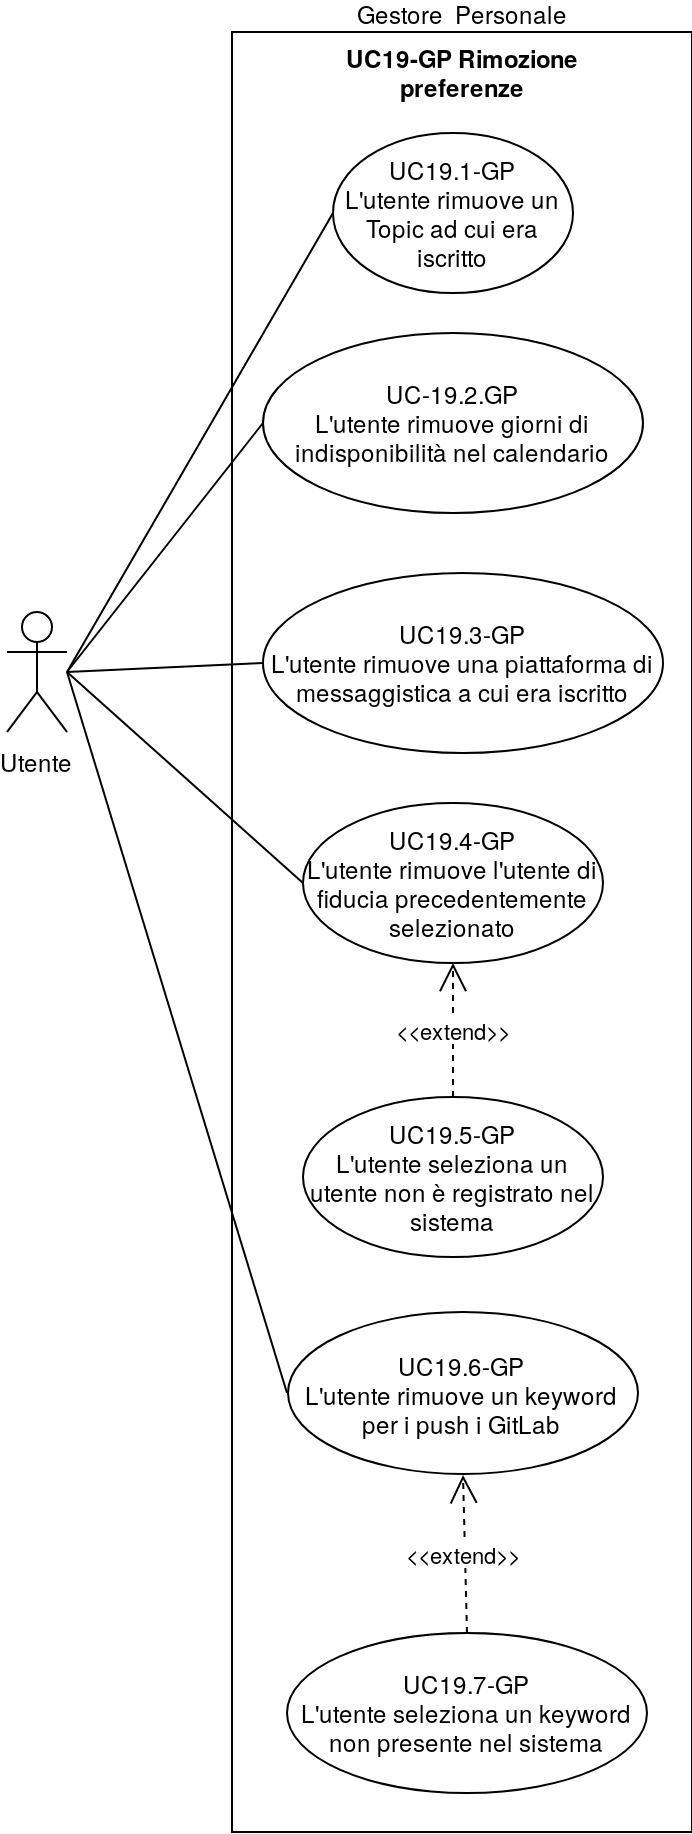
\includegraphics[width=\textwidth]{img/casi_d'uso/UC19.png}\\
			\caption{UC\theuccount-GP - Rimozione preferenze}
		\end{figure}
	\begin{itemize}
		\item \textbf{Codice}: UC\theuccount-GP.
		\item \textbf{Titolo}: rimozione preferenze.
		\item \textbf{Attori primari}: utente.
		\item \textbf{Descrizione}: l’utente, dopo aver selezionato delle preferenze dalle opzioni di configurazione, ne rimuove una o più. Le preferenze consistono in Topic, date di calendario, piattaforma di messaggistica (Telegram e email) e persona di fiducia che lo può sostituire.
		\item \textbf{Precondizione}: l’utente ha eseguito l'accesso nel sistema ed è presente almeno	una preferenza selezionata tra quelle proposte da Butterfly.
		\item \textbf{Postcondizione}: la nuova configurazione contiene una o più preferenze in meno rispetto	a quella precedente.
		\item \textbf{Scenario Principale}:
		\begin{enumerate}
			\item L'utente procede alla rimozione di una o più preferenze
		\end{enumerate}
	\end{itemize}

	\stepcounter{subuccount}
	\paragraph{UC\theuccount.\thesubuccount-GP - Disiscrizione Topic}
		
		\begin{itemize}
			\item \textbf{Codice}: UC\theuccount.\thesubuccount-GP.
			\item \textbf{Titolo}: disiscrizione Topic.
			\item \textbf{Attori primari}: utente.
			\item \textbf{Descrizione}: l’utente si disiscrive da uno o più Topic dai quali prima riceveva delle notifiche.
			\item \textbf{Precondizione}: l’utente ha acceduto correttamente nel sistema e non ha già selezionato tutti i Topic possibili proposti da \progetto.
			\item \textbf{Postcondizione}: il numero di Topic a cui è iscritto l’utente è diminuito.
			\item \textbf{Scenario Principale}:
			\begin{enumerate}
				\item L'utente procede alla disiscrizione di uno o più Topic
			\end{enumerate}
		\end{itemize}
	
	\stepcounter{subuccount}
	\paragraph{UC\theuccount.\thesubuccount-GP - Rimozione di uno o più giorni di irreperibilità nel calendario}
	
	\begin{itemize}
		\item \textbf{Codice}: UC\theuccount.\thesubuccount-GP.
		\item \textbf{Titolo}: rimozione di uno o più giorni di irreperibilità nel calendario.
		\item \textbf{Attori primari}: utente.
		\item \textbf{Descrizione}: l’utente rimuove i giorni di calendario in cui precedentemente	non era reperibile, tornando disponibile.
		\item \textbf{Precondizione}: l’utente ha acceduto correttamente nel sistema ed è presente almeno un giorno di calendario selezionato tra quelli proposti da \progetto.
		\item \textbf{Postcondizione}: il numero di giorni di calendario in cui l’utente non è reperibile è diminuito.
		\item \textbf{Scenario Principale}:
		\begin{enumerate}
			\item L'utente procede alla rimozione di uno o più giorni di irreperibilità
		\end{enumerate}
	\end{itemize}
	
	\stepcounter{subuccount}
	\paragraph{UC\theuccount.\thesubuccount-GP - Rimozione preferenza piattaforma di messaggistica}
	
	\begin{itemize}
		\item \textbf{Codice}: UC\theuccount.\thesubuccount-GP.
		\item \textbf{Titolo}: rimozione preferenza piattaforma di messaggistica.
		\item \textbf{Attori primari}: utente.
		\item \textbf{Descrizione}: l’utente rimuove una o più preferenze tra Telegram e Email dalle	quali non vuole più ricevere notifiche tramite \progetto.
		\item \textbf{Precondizione}: l’utente ha acceduto correttamente nel sistema ed è presente almeno una piattaforma di messaggistica selezionata tra quelle proposte da \progetto.
		\item \textbf{Postcondizione}: il numero di piattaforme di messaggistica da cui l’utente vuole ricevere notifiche è diminuito.
		\item \textbf{Scenario Principale}:
		\begin{enumerate}
			\item L'utente procede alla rimozione di una o più piattaforme di messaggistica
		\end{enumerate}
	\end{itemize}
	
	\stepcounter{subuccount}
	\paragraph{UC\theuccount.\thesubuccount-GP - Rimozione persona di fiducia}
	
	\begin{itemize}
		\item \textbf{Codice}: UC\theuccount.\thesubuccount-GP.
		\item \textbf{Titolo}: aggiunta persona di fiducia.
		\item \textbf{Attori primari}: utente.
		\item \textbf{Descrizione}:  l’utente rimuove l'utente legato a un ID di sua preferenza a cui inoltrare i messaggi in caso di indisponibilità.
		\item \textbf{Precondizione}: l’utente ha eseguito l'accesso nel sistema ed è presente almeno uno user con l'ID selezionato tra quelle proposte da \progetto.
		\item \textbf{Postcondizione}: la preferenza viene rimossa correttamente.
		\item \textbf{Scenario Principale}:
		\begin{enumerate}
			\item L'utente procede alla rimozione della sua persona di fiducia
		\end{enumerate}
		\item \textbf{Estensioni}:
		\begin{enumerate}
			\item Errore ID persona di fiducia inesistente [UC\theuccount.5-GP].
		\end{enumerate}
	\end{itemize}
	
	\stepcounter{subuccount}
	\paragraph{UC\theuccount.\thesubuccount-GP - Errore ID persona di fiducia inesistente}
	
	\begin{itemize}
		\item \textbf{Codice}: UC\theuccount.\thesubuccount-GP.
		\item \textbf{Titolo}: errore ID persona di fiducia inesistente.
		\item \textbf{Attori primari}: utente.
		\item \textbf{Descrizione}: l’utente viene avvisato che ha inserito un identificativo errato.
		\item \textbf{Precondizione}: l’utente ha acceduto con le sue credenziali corrette nel sistema e non ha già selezionato la persona a cui inoltrare le notifiche.
		\item \textbf{Postcondizione}: il sistema comunica all’utilizzatore l’errore di preferenza.
		\item \textbf{Scenario Principale}:
		\begin{enumerate}
			\item L'utente procede alla rimozione della sua persona di fiducia, questa però non esiste e
			visualizza l'errore
		\end{enumerate}
	\end{itemize}

	\stepcounter{subuccount}
	\paragraph{UC\theuccount.\thesubuccount-GP - Rimozione con successo di keyword per i push di GitLab}
	
	\begin{itemize}
		\item \textbf{Codice}: UC\theuccount.\thesubuccount-GP.
		\item \textbf{Titolo}: rimozione con successo di keyword per i push di GitLab.
		\item \textbf{Attori primari}: utente.
		\item \textbf{Descrizione}: l’utente seleziona e rimuove una o più keyword già presente nel sistema per non ricevere la notifica di push in
		cui i messaggi di commit contengono la keyword rimossa.
		\item \textbf{Precondizione}:  l’utente ha acceduto con le sue credenziali corrette nel sistema.
		\item \textbf{Postcondizione}: nelle nuove configurazioni dell'utente selezionato sono state rimosse delle keyword precedentemente presenti.
		\item \textbf{Scenario Principale}:
		\begin{enumerate}
			\item L'utente rimuove con successo una o più keyword per cui non vuole iù ricevere messaggi di push
		\end{enumerate}
		\item \textbf{Estensioni}:
		\begin{enumerate}
			\item Errore keyword da rimuovere non presente [UC\theuccount.7-GP]
		\end{enumerate}
	\end{itemize}
	
	\stepcounter{subuccount}
	\paragraph{UC\theuccount.\thesubuccount-GP - Errore keyword da rimuovere non presente}
	
	\begin{itemize}
		\item \textbf{Codice}: UC\theuccount.\thesubuccount-GP.
		\item \textbf{Titolo}: errore keyword da rimuovere non presente.
		\item \textbf{Attori primari}: utente.
		\item \textbf{Descrizione}: la keyword che l'utente intende rimuovere non è registrata nel sistema.
		\item \textbf{Precondizione}: l’utente ha acceduto con le sue credenziali corrette nel sistema.
		\item \textbf{Postcondizione}: viene visualizzato un messaggio d'errore con indicato che la keyword	selezionata che non è presente nel sistema.
		\item \textbf{Scenario Principale}:
		\begin{enumerate}
			\item L'utente procede alla rimozione di una keyword che non è presente nel sistema e visualizza l'errore
		\end{enumerate}
	\end{itemize}
	

\clearpage